%Chapter 5

\renewcommand{\thechapter}{5}

\chapter{Interlayer exciton and optical nonlinearity of Fermi polaron in Trilayer WSe$_2$}
\label{chap5}

Realizing strong nonlinear optical responses is a long-standing goal of both fundamental and technological importance. Recently significant efforts have focused on exploring excitons in solids to achieve nonlinearities even down to few-photon levels. 
However, a crucial tradeoff arises as strong light-matter interactions require large oscillator strength and short radiative lifetime of excitons, which limits their nonlinearity. 
Here we experimentally demonstrate strong nonlinear optical responses with large oscillator strength by exploiting the coupling between excitons and carriers in an atomically thin semiconductor. 
By controlling the electric field and electrostatic doping of trilayer $WSe_2$, we observe the hybridization between intralayer and interlayer excitons and the formation of Fermi polarons. 
Substantial optical nonlinearity is observed under continuous wave and pulsed laser excitation, where the Fermi polaron resonance blueshifts by as much as ~10 meV. 
Intriguingly, we observe a remarkable asymmetry in the optical nonlinearity between electron and hole doping, which is tunable by the applied electric field.
We attribute these features to the optically induced valley polarization due to the interactions between excitons and free charges. 
Our results establish atomically thin heterostructures as a highly versatile platform for engineering nonlinear optical response with applications to classical and quantum optoelectronics.

\section{Introduction}
Nonlinear optical phenomena lie at the heart of classical and quantum optics, with applications ranging from data communications to quantum control\cite{Volz2012-pb,Boyd2020-re}. 
Developing physical systems with stronger optical nonlinearity while reducing their power requirement holds the promise for more efficient optoelectronics and may unlock new technologies such as single-photon switches and transistors\cite{}. 
In recent years, significant efforts have been devoted to investigating excitons in semiconductors as a solid-state medium for realizing strong optical nonlinearity1–3.
Van der Waals heterostructures based on atomically thin transition metal dichalcogenides (TMDs) have emerged as a new platform for fundamental studies of excitons and for engineering optical responses9,10. Excitons in such two-dimensional materials are highly tunable with rich spin-valley physics and possess characteristics promising for optical nonlinearity, such as strong light-matter interactions and weak screening of Coulomb potential10. 
However, a major challenge in achieving high nonlinearity under low excitation power arises from the balance between the strengths of exciton-photon and exciton-exciton interactions11–13. 
For instance, intralayer excitons in these materials exhibit large oscillator strength but experience weak interactions, dominated by exchange interactions and limited by their short lifetime14. 
On the other hand, interlayer excitons in TMD heterostructures have longer lifetimes and experience interactions due to their finite electric dipole moment15,16. 
Unfortunately, spatial separation of the electron-hole wavefunctions leads to weaker absorption of incident photons. 
Several recent studies demonstrated enhanced the interlayer exciton absorption via its hybridization with intralayer excitons in $MoS_2$1,17–19, although the oscillator strength of such hybrid excitons is still an order of magnitude weaker than the intralayer ones. 
So far, strong nonlinearity in the intralayer excitons has not yet been realized.
In this study, we report giant nonlinear optical responses of intralayer charged excitons, i.e., Fermi polarons, on the order of several millielectronvolts under photon flux of 1013 photons per second per square micrometer. 
The strong nonlinearity is highly tunable by doping and electric field, based on which we attribute the nonlinearity to an optically induced valley polarization resulting from exciton-carrier scattering.

\section{Sample Fabrication}
Graphite, hBN flakes are mechanically exfoliated from the bulk crystals onto the silicon chip with $SiO_2$ layer. 
Some of the exfoliated homotrilayer $WSe_2$ flakes were provided by the Quantum material press (QPress) facility in Center for functional nanomaterials (CFN) at Brookhaven national laboratory (BNL). 
The thickness of the hBN flakes and $WSe_2$ layer numbers are estimated based on the color contrast under the optical microscopy. 
The heterostructure is assembled in a transfer station built by Everbeing Int’l Corp., which use PDMS(Polydimethylsiloxane) and PC (Polycarbonate) as stamp and transfer all the flakes in a dry transfer method onto a silicon chip with 285nm $SiO_2$ layer. 
Then the electrical contacts are patterned by electron-beam lithography and a liftoff process where we deposited 5nm of Cr and 80 nm of Au by thermal evaporation.
Figure~\ref{fig.5.1} shows the device schematic and the fabricated device optical image under 100 X magnification. 

%////////////////////////////Figure Panel//////////////////
%Fig.5.1--------------
\renewcommand{\baselinestretch}{1}
\small\normalsize
\begin{quote}
\begin{figure}
\begin{center}
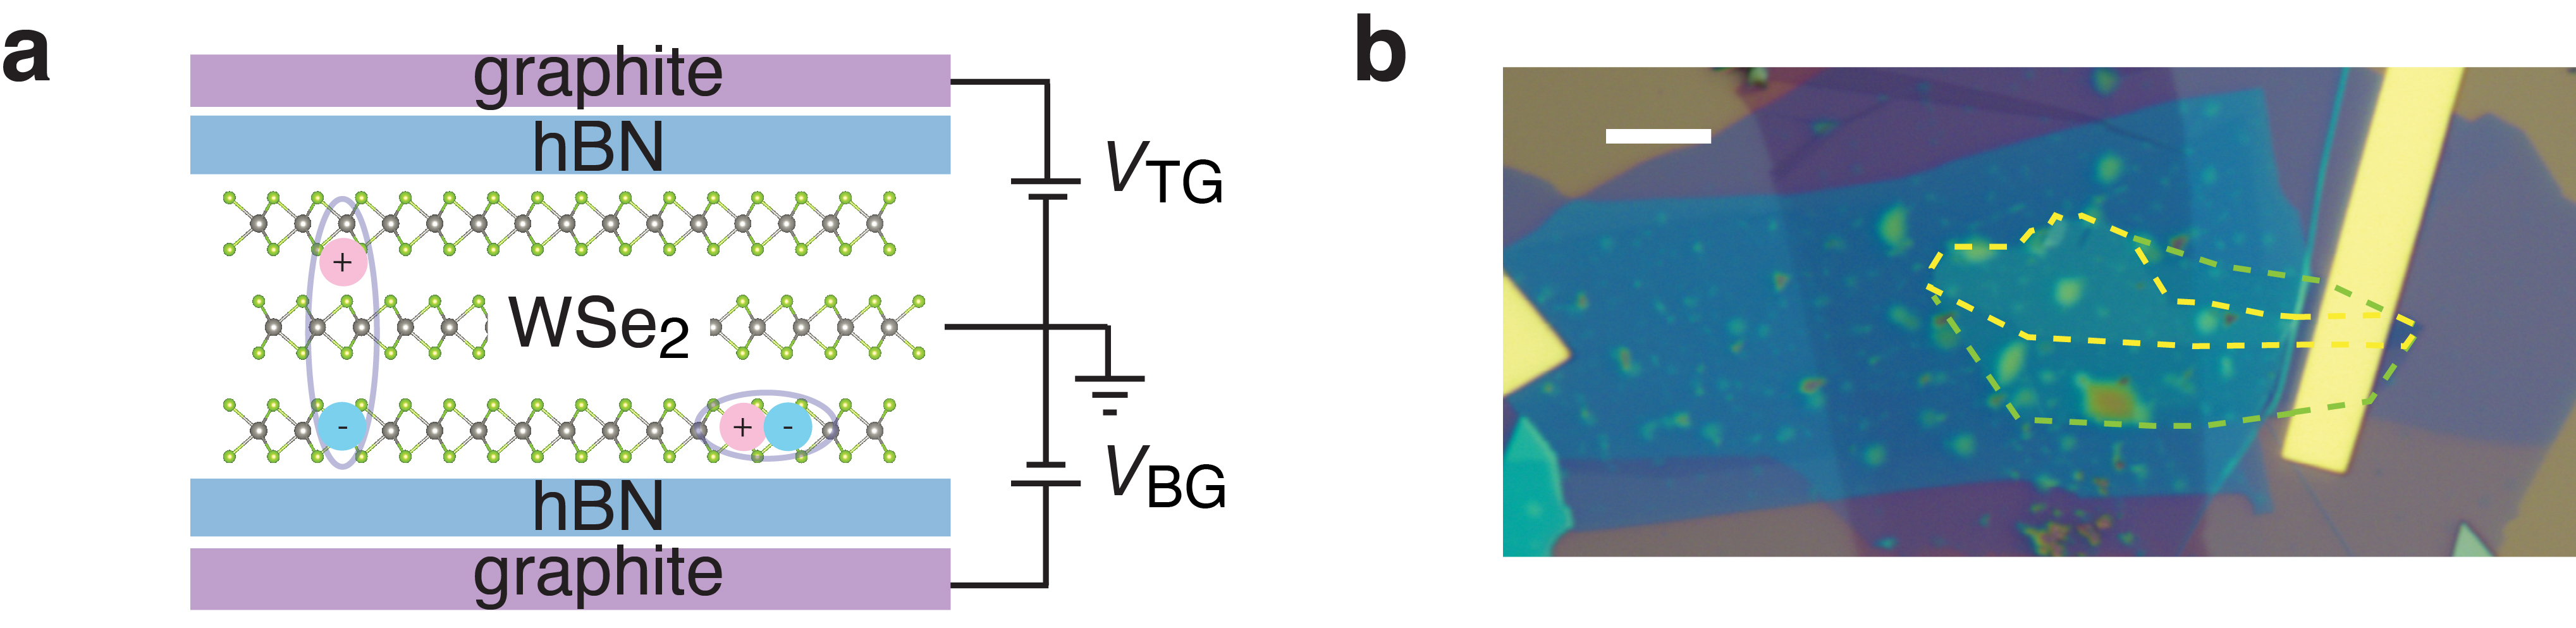
\includegraphics[width=1\textwidth]{Figures/C5/Fig5_1.jpg} % 
\end{center}
\caption[Dual-gated WSe$_2$ homotrilayer van der Waals heterostructure] {\textbf{Dual-gated WSe$_2$ homotrilayer van der Waals heterostructure.} \textbf{a}, Schematic of the trilayer vdW heterostructure. 
The homotrilayer WSe$_2$ is encapsulated with two hBN layers of thickness 15-20 nm. 
\textbf{b}, Optical image of the homotrilayer WSe$_2$ device (scale bar: 5~$\mu$m). 
The trilayer and neighboring bilayer regions are enclosed by yellow and green dashed lines, respectively.}
\label{fig.5.1}
\end{figure}
\end{quote}
\renewcommand{\baselinestretch}{2}
\small\normalsize
% %///////////////////////
\section{Results and Discussions}
\subsection{Electrical control of excitons}
In our experiments, we encapsulate exfoliated WSe$_2$ homotrilayers inside two layers of hBN in a dual-gate geometry to independently control the overall doping levels and the displacement field (Figure~\ref{fig.5.2}). 
Figure~\ref{fig.5.2}a shows the photoluminescence (PL) map of the sample by varying the electric field while keeping the samples undoped. 
We observe strong emission from excitons XI, whose energy linearly shifts with electric field from 1.58 eV to 1.50 eV, and PL peaks at 1.71, 1.55 and 1.52 eV that remains constant with varying electric field. 
We attribute the peak at 1.71 eV to intralayer momentum-direct exciton X$_A$ at the K-K transition, based on their strong absorption (Figure~\ref{fig.5.2}b) and zero Stark shift. 

%////////////////////////////Figure Panel//////////////////
%Fig.5.2--------------
\renewcommand{\baselinestretch}{1}
\small\normalsize
\begin{quote}
\begin{figure}
\begin{center}
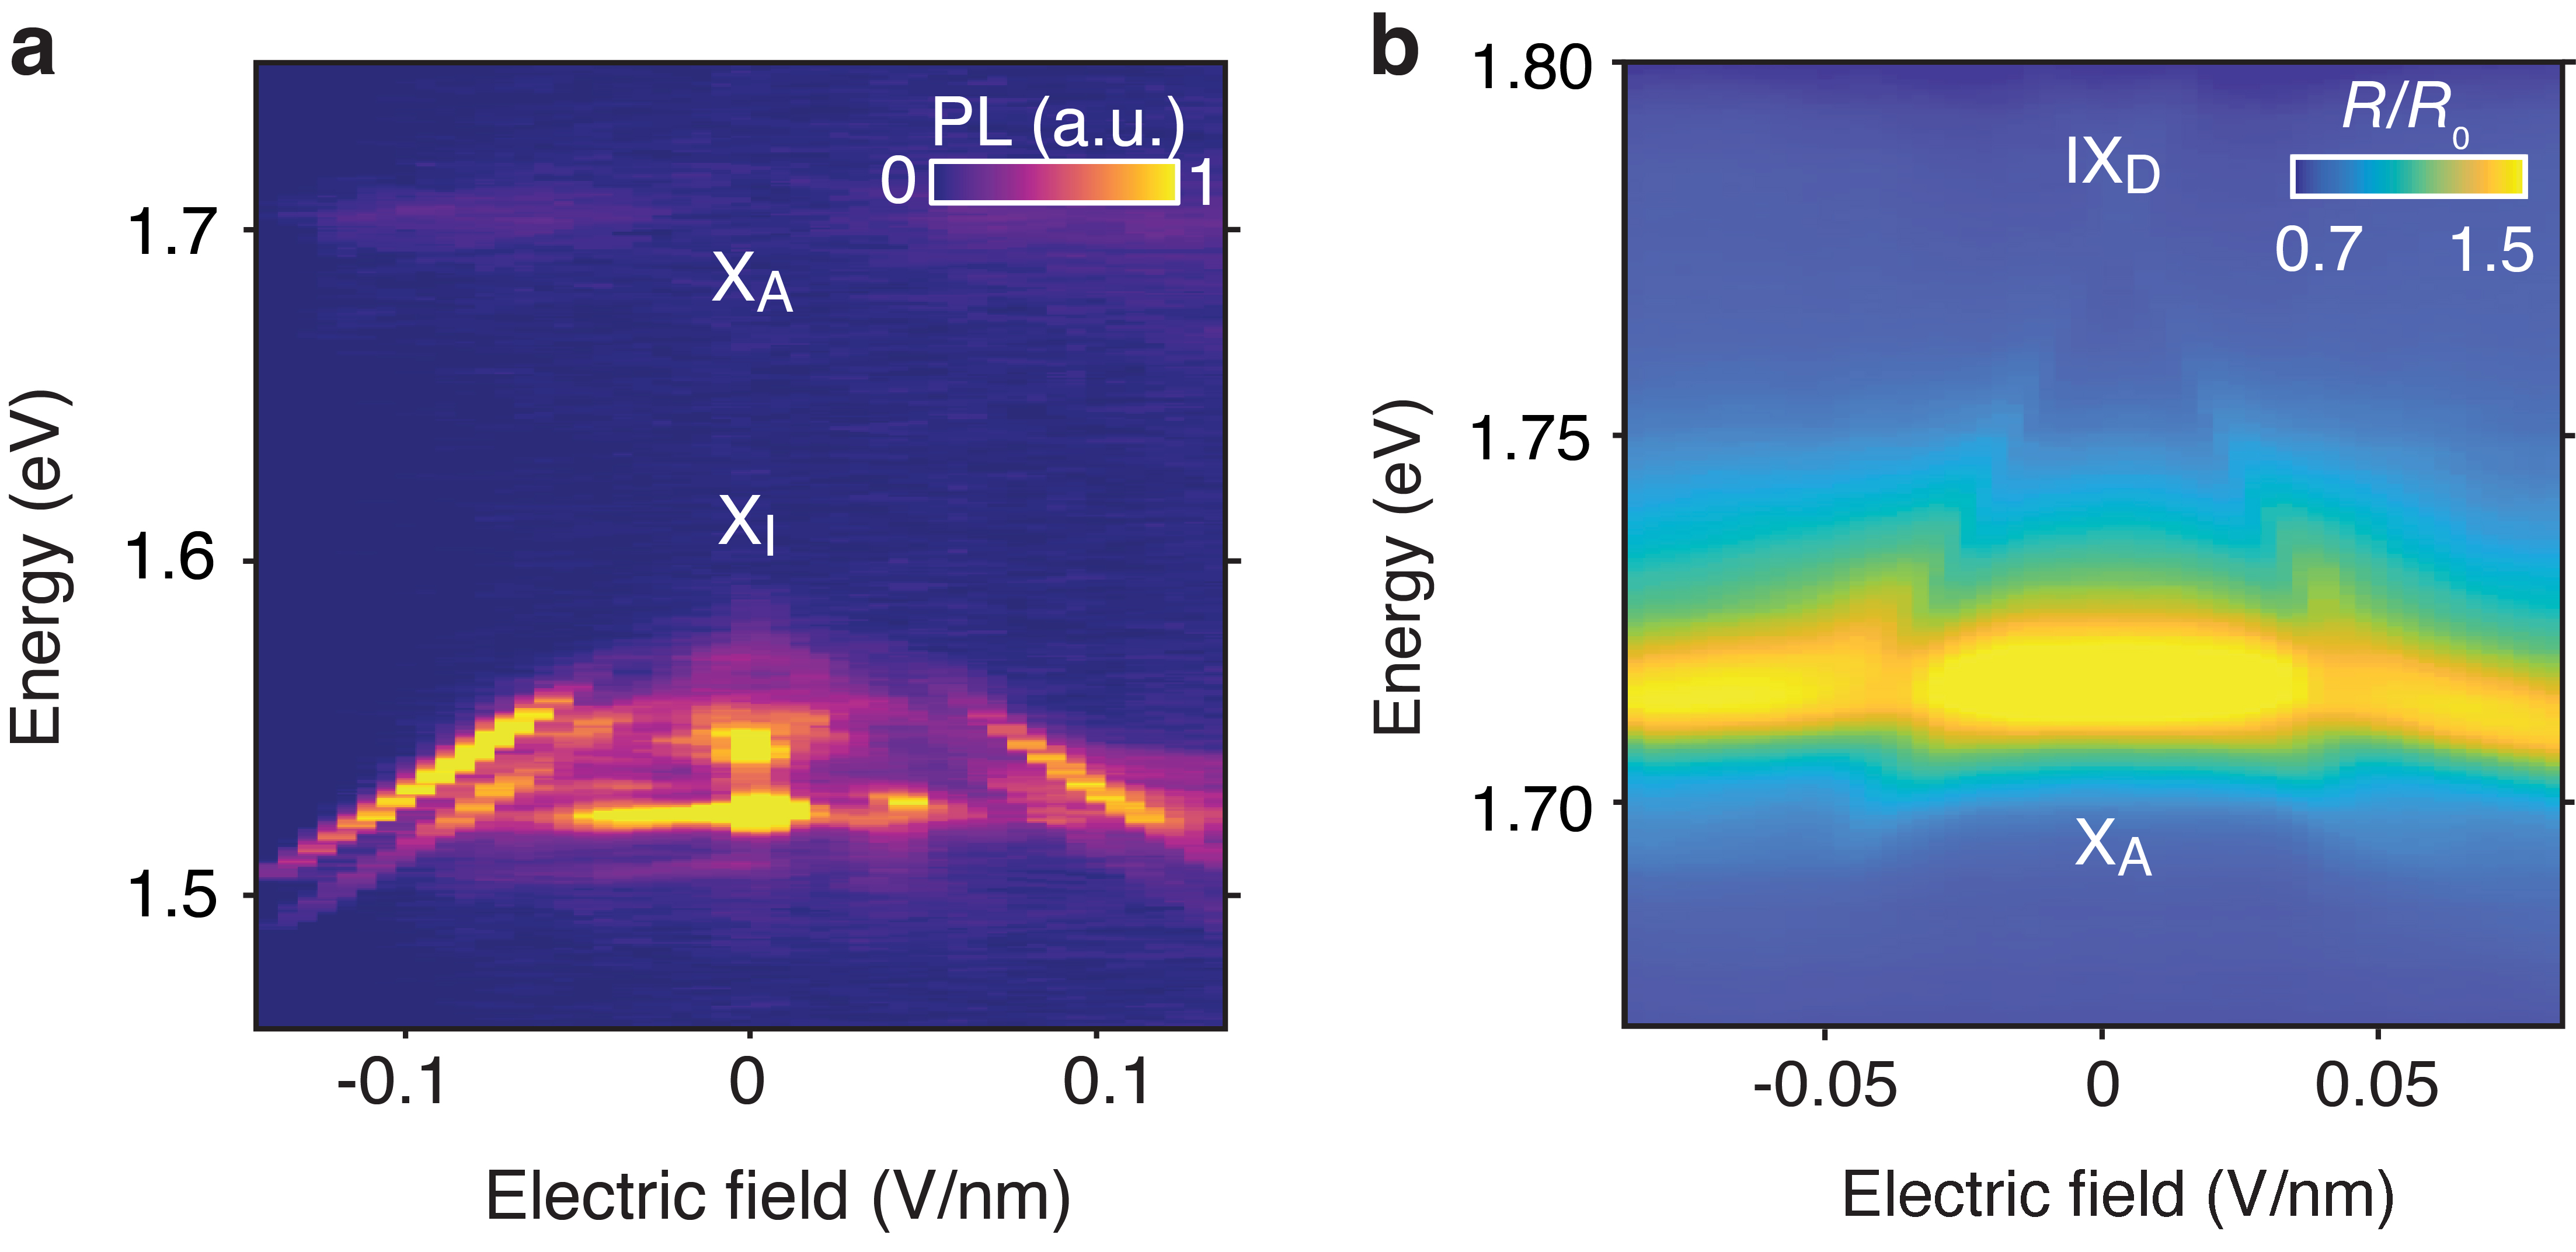
\includegraphics[width=0.85\textwidth]{Figures/C5/Fig5_2.jpg} % 
\end{center}
\caption[Optical characteristic of dual-gated homotrilayer WSe$_2$ van der Waals heterostructure.] {\textbf{Optical characteristic of dual-gated homotrilayer WSe$_2$ van der Waals heterostructure.} 
\textbf{a}, Photoluminescence spectra of the WSe$_2$ trilayer under an applied electric field. 
The bright emission at 1.50--1.58~eV, exhibiting a Stark shift with field, corresponds to the indirect exciton X$_I$. 
The weaker emission near 1.70~eV corresponds to the momentum-direct K--K intralayer exciton X$_A$.  
\textbf{b}, Reflectance spectra of the WSe$_2$ trilayer under an electric field. 
The high-energy momentum-direct K--K interlayer exciton exhibits a Stark shift of $\sim$100~meV and begins to hybridize with X$_A$ when their energies become degenerate around an electric field of $\sim$ 0.05 V/nm.}
\label{fig.5.2}
\end{figure}
\end{quote}
\renewcommand{\baselinestretch}{2}
\small\normalsize
% %///////////////////////

The lower energy of X$_I$ indicates that they are momentum-indirect excitons at the band edge, corresponding to transition across the indirect gap, located at the valence band $\Gamma$ and conduction band Q valleys, according to the band structure calculations20–22. 
From the linear Stark shift, we estimate the electric dipole of X$_I$.  
The energy shift as a function of the electric field of the IX$_D$ and X$_I$ obeys the law of the stark shift, which can be described as:
\begin{equation}
\Delta E = \lvert e \cdot d \cdot E \rvert 
= \left\lvert e \cdot d \cdot \frac{\varepsilon_{\mathrm{hBN}}}{\varepsilon_{\mathrm{WSe_2}}}
\cdot \frac{V_{\mathrm{BG}}}{t_{\mathrm{BG}}} \right\rvert 
\label{eq:deltaE}
\end{equation}
Thus the dipole moment of excitons can be calculated as:
\begin{equation}
d = \left\lvert 
\frac{\Delta E}{e} \cdot 
\frac{\varepsilon_{\mathrm{WSe_2}}}{\varepsilon_{\mathrm{hBN}}} \cdot 
\frac{t_{\mathrm{BG}}}{V_{\mathrm{BG}}} 
\right\rvert
\label{eq:d_expression}
\end{equation}
The estimated electric dipole of X$_I$ is around 0.78 $nm\cdot e$. 
The corresponding vertical displacement of the electron-hole pair in X$_I$ is approximately half of the distance between the top and bottom tungsten layers, indicating the electrons or holes are partially layer delocalized. 

Next, we measure the reflectance of the trilayer under an electric field (Figure~\ref{fig.5.2}b). 
In addition to the intralayer X$_A$, we observe an additional reflectance contrast at 1.78 eV (IX$_D$), which exhibits a substantial Stark effect of almost 100 meV (additional devices shown in Figure~\ref{fig.5.2}). 
The finite reflection contrast and linear Stark effect of IX$_D$ suggest that it corresponds to interlayer exciton at the direct K-K transition with larger oscillator strength than those momentum-indirect excitons, X$_I$, observed in PL.
From the slope of the Stark effect, we estimate the electron-hole displacement to be 1.35 $nm$. 
Interestingly, as the energy of IX$_D$ approaches that of the intralayer exciton X$_A$ under a higher electric field, we observe an apparent anti-crossing behavior of X$_A$ and IX$_D$ near the electric field of 0.05 V/nm. 
We note that the levels are not fully avoided and there is always finite reflection from X$_A$ at 1.71 eV for all electric fields, which will be discussed in more depth later. 

%////////////////////////////Figure Panel//////////////////
%Fig.5.3--------------
\renewcommand{\baselinestretch}{1}
\small\normalsize
\begin{quote}
\begin{figure}
\begin{center}
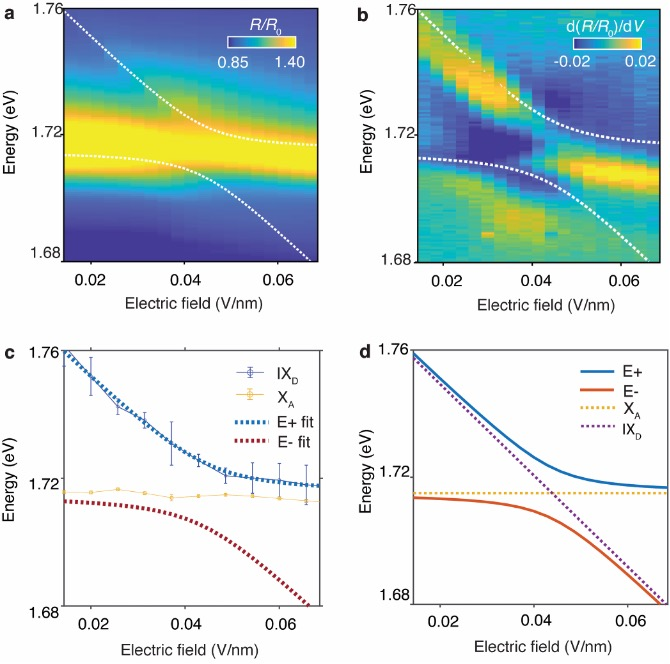
\includegraphics[width=0.8\textwidth]{Figures/C5/Fig5_3.jpg} % 
\end{center}
\caption[Analysis of anti-crossing between IX$_D$ and X$_A$ in device D1.] {\textbf{Analysis of anti-crossing between IX$_D$ and X$_A$ in device D1.} 
\textbf{a}, Reflectance spectra ($R/R_{0}$) as a function of the electric field near the anti-crossing region.  
\textbf{b}, Voltage derivative of reflectance spectra, $d(R/R_{0})/dV$.  
The white dashed lines in \textbf{(a)} and \textbf{(b)} represent the energies fitted with a two-level model.  
\textbf{c}, Fitted anti-crossing between the IX$_D$ and X$_A$.  
The solid lines with error bars in \textbf{(c)} denote the fitted peak energies of IX$_D$ (blue) and X$_A$ (yellow) extracted with Lorentzian fits to the spectra.  
The dotted line shows the IX$_D$ branch obtained from the coupled oscillator model.  
Error bars represent the variance of the fitted peak energies.  
\textbf{d}, Simulated two-level anti-crossing.}
\label{fig.5.3}
\end{figure}
\end{quote}
\renewcommand{\baselinestretch}{2}
\small\normalsize
% %///////////////////////
To quantitatively understand the avoided crossing, we extract the exciton energies by fitting reflectance spectra and then model the anti-crossing based on a two-level system with a Hamiltonian:
\begin{equation}
H =
\begin{pmatrix}
E_{1} & W \\
W & E_{2}
\end{pmatrix}
\label{eq:Hamiltonian}
\end{equation}
where $E_{1}$ and $E_{2}$ are the unperturbed energies of the IX$_{D}$ and X$_{A}$, respectively, and $W$ is the coupling strength. The new eigenvalues can be expressed as:
\begin{equation}
E_{\pm} = \frac{1}{2}(E_{1}+E_{2})
\pm \frac{1}{2}\sqrt{(E_{1}-E_{2})^{2}+4\lvert W\rvert^{2}}
\label{eq:eigenvalues}
\end{equation}
where $E_{\pm}$ correspond to the energies of the two branches.  
In Figures~\ref{fig.5.3}c, we extract the peak positions $E_{\pm}$ by fitting the reflectance spectra with Lorentzian functions.  
We then set $E_{2} = 1.715~\text{eV}$, corresponding to the mean energy of X$_A$, and keep it constant.  
$E_{1}$ is calculated based on the IX$_D$ energy at zero electric field and its Stark shift.  
The Stark shift slope $k$ is estimated to be $-1.436~\text{eV/V}$ for this device. 
The fitted anti-crossing is shown in Figures~\ref{fig.5.3}c,d, yielding a coupling parameter of $W = 10 \pm 2~\text{meV}$ between X$_A$ and IX$_D$. 

%////////////////////////////Figure Panel//////////////////
%Fig.5.4--------------
\renewcommand{\baselinestretch}{1}
\small\normalsize
\begin{quote}
\begin{figure}
\begin{center}
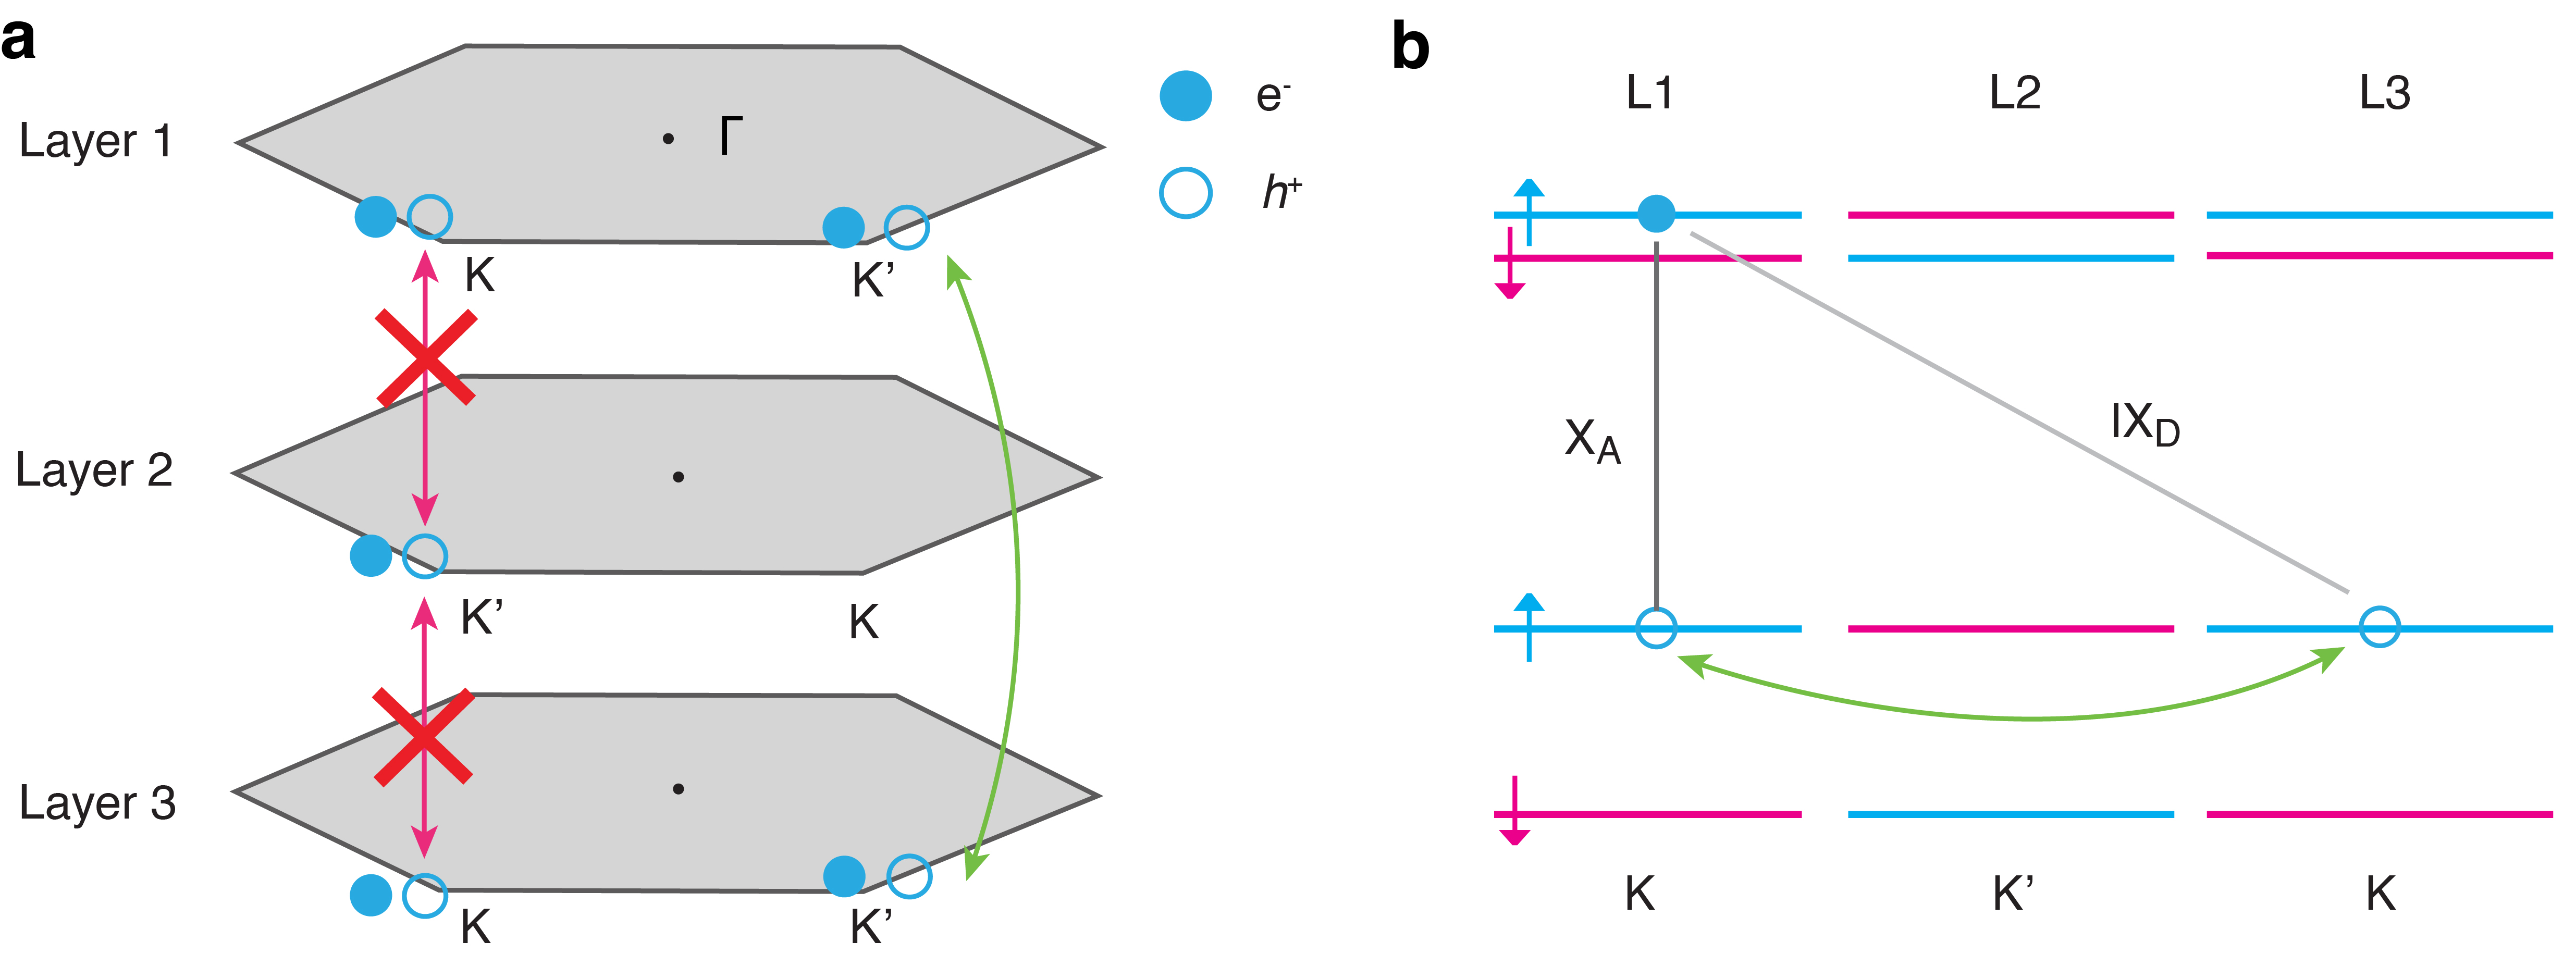
\includegraphics[width=0.9\textwidth]{Figures/C5/Fig5_4.jpg} % 
\end{center}
\caption[Electronic band structure of trilayer WSe$_2$.] 
{\textbf{Electronic band structure of trilayer WSe$_2$.} 
\textbf{a}, The crystal structure of natural trilayer WSe$_2$ dictates alternating $K$ and $K'$ valleys among neighboring layers.  
The strong spin--orbit coupling of holes leads to weak tunneling between neighboring layers but strong tunneling between the top and bottom layers.  
\textbf{b}, Hole tunneling between the top and bottom layers results in the hybridization of intralayer $K$--$K$ excitons X$_A$ and interlayer $K$--$K$ excitons IX$_D$. }
\label{fig.5.4}
\end{figure}
\end{quote}
\renewcommand{\baselinestretch}{2}
\small\normalsize
% %///////////////////////

The observed Stark effect and anti-crossing in WSe$_2$ trilayers can be understood by examining their crystal and band structure. 
In trilayers, each monolayer is rotated by $180^{\circ}$, resulting in alternating $K$ and $K'$ points between layers~\cite{ref27} (Figures~\ref{fig.5.4}a,b). 
Here we mainly consider the hole tunneling process, which is predicted to be much stronger than electron tunneling according to density functional theory calculations~\cite{ref28}. 
The sizeable spin--orbit coupling in the valence band dictates that direct tunneling between neighboring layers is much weaker than tunneling between the top and bottom layers across the middle layer (Figures~\ref{fig.5.4}a,b). 
Such tunneling gives rise to finite oscillator strength of interlayer $K$--$K$ excitons (IX$_D$) and their avoided crossing with intralayer excitons X$_A$~\cite{ref29}. 
Indeed, the experimentally extracted coupling strength between X$_A$ and IX$_D$ is consistent with the calculated interlayer hole tunneling strength at the $K$ valley~\cite{ref22}. 
This picture is further supported by our measured dipole moment of IX$_D$, which is close to the distance between the top and bottom layers, and it explains our observation that the level crossing at X$_A$ is not fully avoided, since IX$_D$ does not couple to intralayer excitons in the middle layer.

%////////////////////////////Figure Panel//////////////////
%Fig.5.5--------------
\renewcommand{\baselinestretch}{1}
\small\normalsize
\begin{quote}
\begin{figure}
\begin{center}
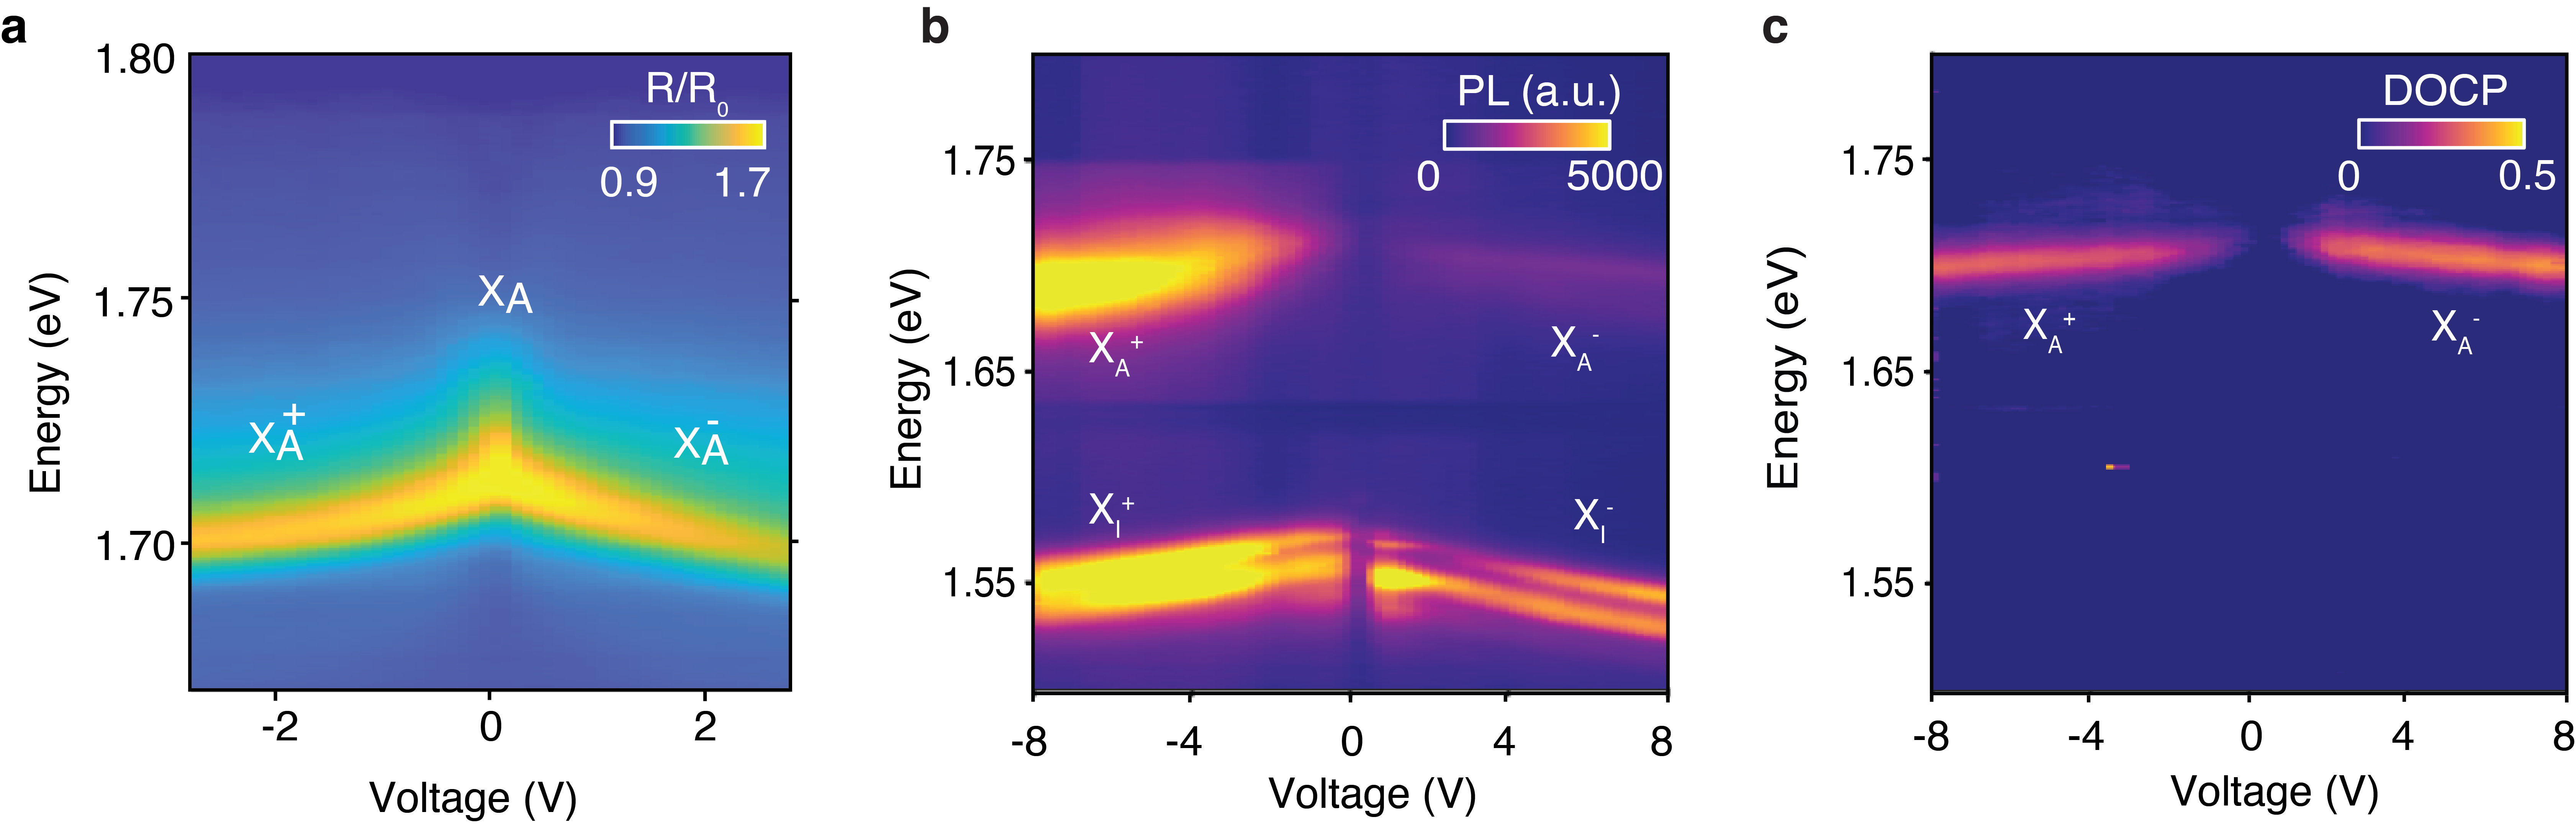
\includegraphics[width=1\textwidth]{Figures/C5/Fig5_5.jpg} % 
\end{center}
\caption[Doping-dependent optical characteristics of trilayer WSe$_2$ at 4~K.] 
{\textbf{Doping-dependent optical characteristics of trilayer WSe$_2$ at 4~K.} 
\textbf{a}, Doping-dependent reflectance spectra of the WSe$_2$ trilayer at 4~K, measured from device D1. 
With increasing doping concentration, the intralayer trion or Fermi polaron (X$_A^-$ / X$_A^+$) shifts toward lower energy.  
\textbf{b}, Doping-dependent photoluminescence of the trilayer WSe$_2$ at $E_z = 0$, measured from device D2 at 4~K under above-band excitation with a 635~nm diode laser.  
\textbf{c}, Degree of circular polarization (DOCP) of the X$_A^+$ and X$_A^-$. 
The bright emission in the range of 1.5--1.6~eV corresponds to the momentum-indirect trion/Fermi polaron, whereas the higher-energy emission around 1.7~eV corresponds to the momentum-direct ($K$--$K$) intralayer trion/Fermi polaron.  
Both charged excitons X$_I$ and X$_A$ exhibit a redshift with increasing doping density.  
}
\label{fig.5.5}
\end{figure}
\end{quote}
\renewcommand{\baselinestretch}{2}
\small\normalsize
% %///////////////////////
We further characterize how electrostatic gating modifies intralayer excitons X$_A$ and their hybridization with interlayer excitons. 
Figure~\ref{fig.5.5}a shows the doping-dependent reflectance spectra of the sample under zero electric field. 
Upon doping, the reflectance from neutral X$_A$ diminishes as they lose oscillator strength, while charged intralayer excitons emerge and shift to lower energies, with similar behavior observed in photoluminescence (PL) (Figure~\ref{fig.5.5}b). 
The redshift of charged excitons with increasing doping can be explained in terms of attractive Fermi polarons~\cite{ref23}, or by an increase in the exciton--trion energy splitting with increasing Fermi energy~\cite{ref24}. 
The similar doping dependence of reflectance and PL arises from the absence of Pauli blocking in both cases when the free carriers do not occupy the $K$ valley~\cite{ref25}. 
As we focus on the highly doped regime where excitons interact with a large number of carriers, we refer to these charged excitons as Fermi polarons in later discussions~\cite{ref23}.

\subsection{Giant optical nonlinearity of Fermi polaron}
Next, we study the nonlinear optical response of excitons by measuring the sample’s reflectance spectra under different laser pumping conditions.
Figures~\ref{fig.5.6}a--c show the reflectance spectra of the sample, probed with a halogen lamp, while being excited with a 635~nm continuous-wave (CW) laser of varying power. 
When the trilayers are electron-doped or intrinsic, optical pumping does not significantly alter the reflectance spectra. 
Intriguingly, however, in the hole-doped regime, optical pumping leads to a pronounced blueshift of the Fermi polaron X$_A^+$, on the order of a few meV, accompanied by a slight linewidth increase under tens of microwatts of excitation (Figure~\ref{fig.5.6}b). 
The oscillator strength of X$_A^+$, extracted from the reflectance spectra, remains nearly constant at low excitation power but decreases at higher power. 
We note that the PL signals are more than four orders of magnitude weaker than the reflected light and are therefore negligible.

%////////////////////////////Figure Panel//////////////////
%Fig.5.6--------------
\renewcommand{\baselinestretch}{1}
\small\normalsize
\begin{quote}
\begin{figure}
\begin{center}
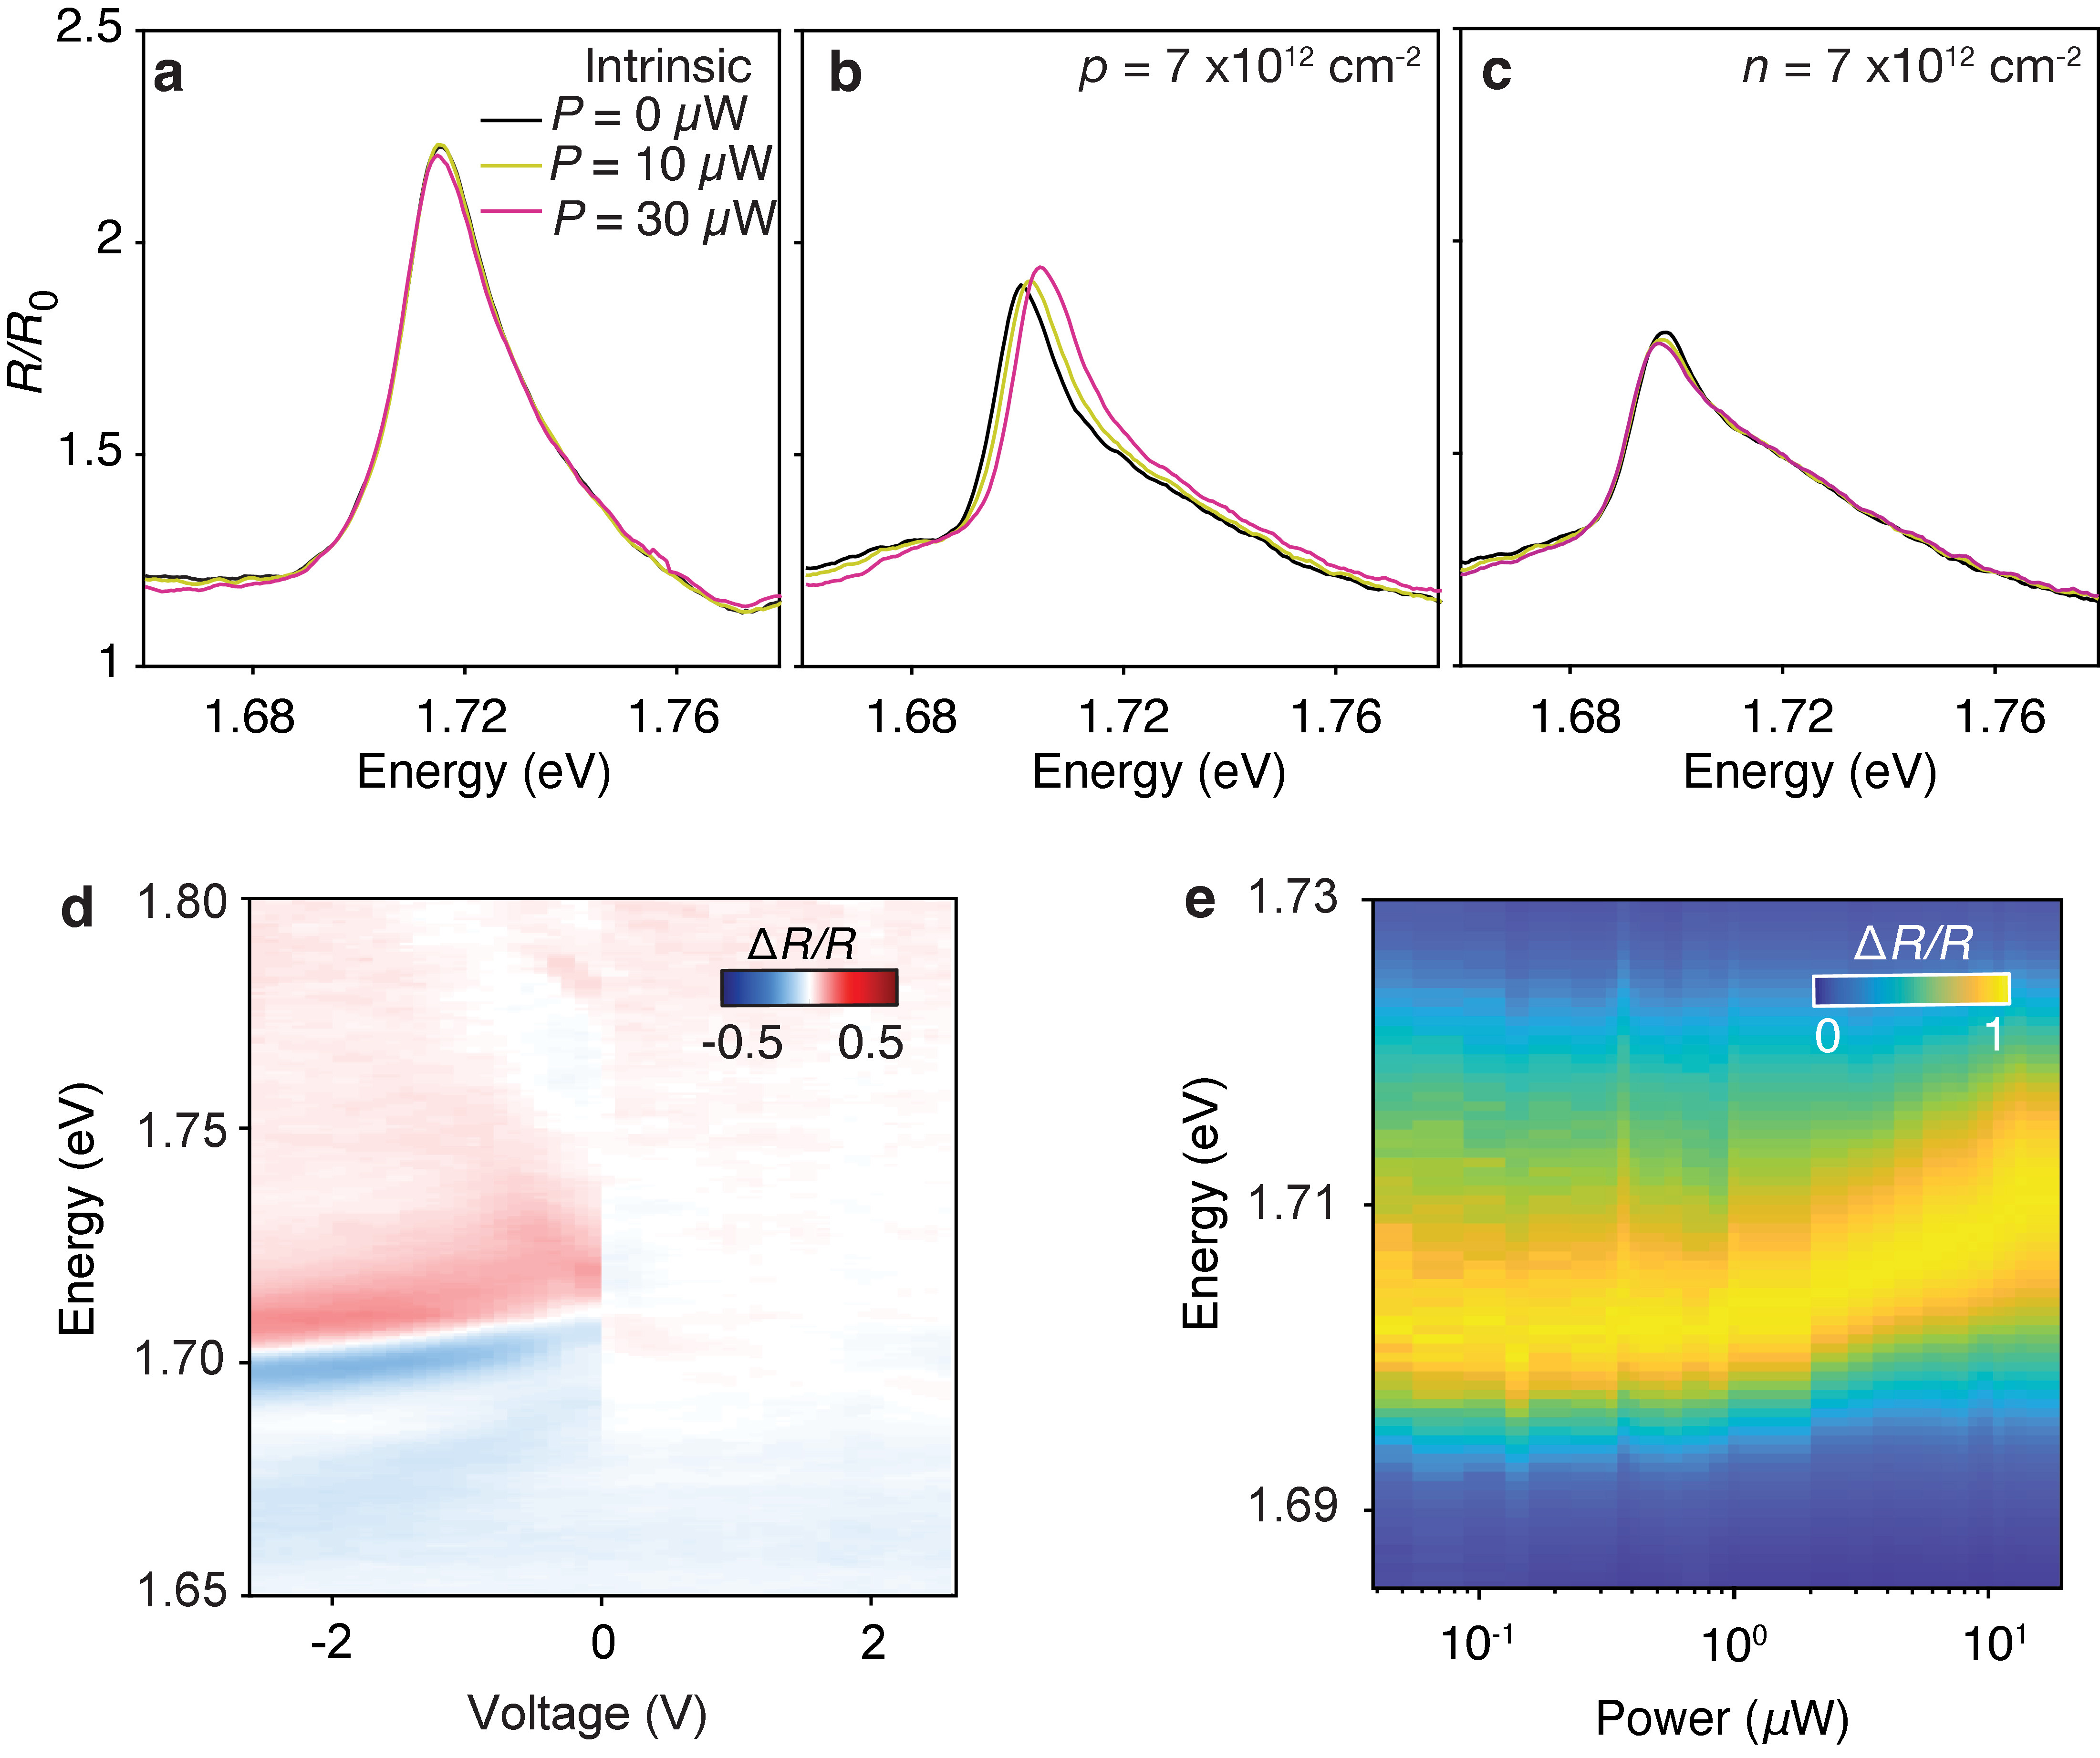
\includegraphics[width=0.85\textwidth]{Figures/C5/Fig5_6.jpg} % 
\end{center}
\caption[Nonlinearity in hole-doped homotrilayer WSe$_2$ at $T = 4$~K.] 
{\textbf{Nonlinearity in hole-doped homotrilayer WSe$_2$ at $T = 4$~K.} 
\textbf{a--c}, Reflectance contrast $R/R_{0}$ of the trilayer under 0~$\mu$W, 10~$\mu$W, and 30~$\mu$W CW (635~nm) laser excitation at different doping levels, where $R_{0}$ is the reflectance of a reference region near the trilayer (bare graphite/hBN/graphite on SiO$_2$). 
Intriguingly, the exciton blueshifts when the sample is hole-doped.  
\textbf{d}, Relative change in reflectance induced by 30~$\mu$W of CW laser pumping under different doping conditions. 
The color map is obtained by normalizing the reflectance with optical pumping to that without optical pumping,  
$\frac{\Delta R}{R} = \frac{R_{30\,\mu\mathrm{W}}}{R_{\mathrm{NoPump}}} - 1$.
Therefore,a positive value (red) at higher energies and a negative value (blue) at lower energies indicate a blueshift. 
The apparent discontinuity near 0~V is due to the high excitation power and finite voltage step used.  
\textbf{e}, Blueshift of X$_A^+$ as a function of pulsed laser excitation power (718--720~nm, resonant with X$_A^+$) at a hole density of $7 \times 10^{12}$~cm$^{-2}$. 
The apparent redshift in the peak energy below 1~$\mu$W is due to fluctuations; in fact, X$_A^+$ consistently shifts toward higher energy with increasing power.}
\label{fig.5.6}
\end{figure}
\end{quote}
\renewcommand{\baselinestretch}{2}
\small\normalsize
%////////////////////////////Figure Panel//////////////////

% To visualize the doping dependence of the nonlinearity, we measure the relative change in the sample’s reflectance induced by optical pumping,  
% $\frac{\Delta R}{R} = \frac{R_{p}}{R_{np}} - 1$,
% where $R_{p}$ and $R_{np}$ are the sample’s reflectance spectra with and without laser pumping, respectively. 
% Figure~5.6d shows $\Delta R / R$ under symmetric gating with zero electric field, where we observe a striking asymmetry between the electron- and hole-doped regimes. 
% We briefly note that the observed nonlinearity of intralayer excitons is orders of magnitude stronger than that of dipolar interlayer excitons in bilayer TMDs~\cite{ref19,ref26} (see Table~S1 for a detailed comparison with other systems). 
% Another critical distinction is that the nonlinearity in bilayer TMDs occurs for interlayer excitons in the intrinsic regime~\cite{ref1,ref19}.
%////////////////////////////Figure Panel//////////////////
%Fig.5.7--------------
\renewcommand{\baselinestretch}{1}
\small\normalsize
\begin{quote}
\begin{figure}
\begin{center}
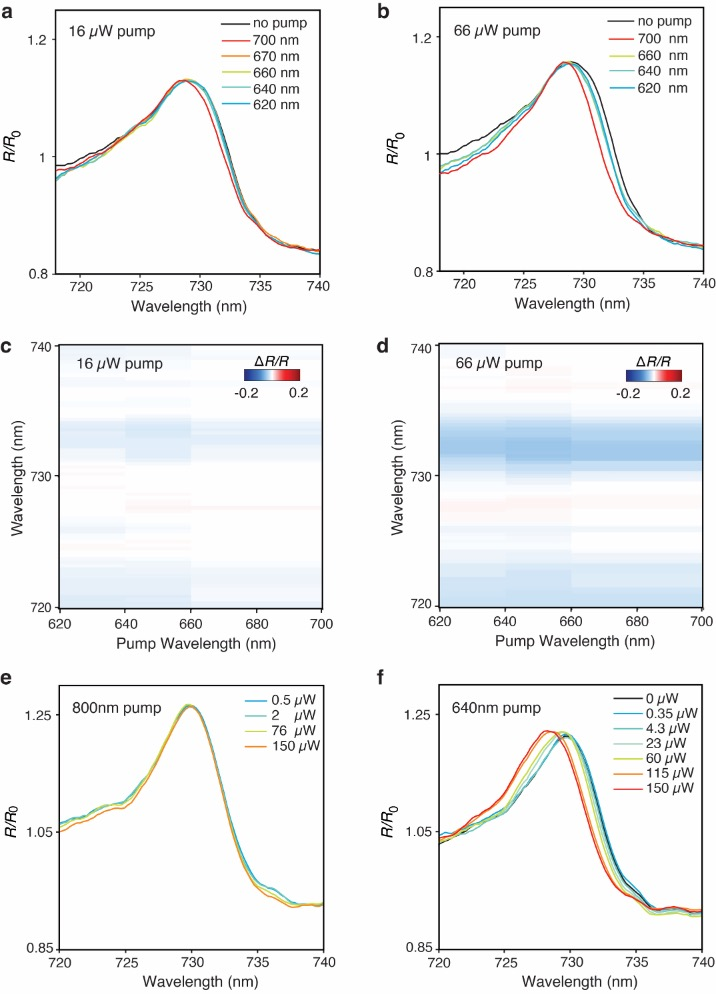
\includegraphics[width=0.7\textwidth]{Figures/C5/Fig5_7.jpg} % 
\end{center}
\caption[Effect of pumping photon energy on nonlinearity.] 
{\textbf{Effect of pumping photon energy on nonlinearity.}
\textbf{a, b,} Blueshift of X$_A^+$ under laser excitation at different center wavelengths ($\sim$10~nm spectral width) with a fixed pumping power at \textbf{(a)} 16~$\mu$W and \textbf{(b)} 66~$\mu$W. 
\textbf{c, d,} The corresponding reflectance changes induced by optical pumping at different wavelengths show no significant wavelength dependence. 
\textbf{e, f,} when exciting the system with photon energies below X$_A^+$, we did not observe significant blueshift \textbf{(e)}, in contrast to higher energy excitation at 640~nm \textbf{(f)}. 
All data is acquired from device D3. We also note that the resonant excitation results in a much more pronounced blueshift.
}
\label{fig.5.7}
\end{figure}
\end{quote}
\renewcommand{\baselinestretch}{2}
\small\normalsize
% %///////////////////////

To visualize the doping dependence of the nonlinearity, we measure the relative change in the sample’s reflectance induced by optical pumping,  
$\frac{\Delta R}{R} = \frac{R_{p}}{R_{np}} - 1$,
where $R_{p}$ and $R_{np}$ are the sample’s reflectance spectra with and without laser pumping, respectively. 
Figure~5.6d shows $\Delta R / R$ under symmetric gating with zero electric field, where we observe a striking asymmetry between the electron- and hole-doped regimes. 
We briefly note that the observed nonlinearity of intralayer excitons is orders of magnitude stronger than that of dipolar interlayer excitons in bilayer TMDs~\cite{ref19,ref26} (see Table~S1 for a detailed comparison with other systems). 
Another critical distinction is that the nonlinearity in bilayer TMDs occurs for interlayer excitons in the intrinsic regime~\cite{ref1,ref19}.

In addition to non-resonant excitation, we also probe the optical nonlinearity by resonantly exciting X$_A$ with a pulsed laser (718--730~nm wavelength, $\sim$100~ps pulse duration), and we observe qualitatively similar nonlinear behavior with a $\sim$10~meV blueshift of X$_A^+$ and a linewidth increase, but only on the hole-doped side(Figure~\ref{fig.5.6}e). 
To investigate how excitation photon energy impacts the nonlinearity, we tune the pulsed laser energy across the X$_A^+$ resonance. 
This resonant excitation results in a stronger blueshift than higher-energy excitation, while no obvious shift in X$_A^+$ is observed when the photon energy falls below X$_A^+$ (Figure~\ref{fig.5.7}). 
Additionally, we find no significant wavelength dependence when the photon energy exceeds X$_A^+$ (Figure~\ref{fig.5.7}). 
Notably, pulsed excitation generates an order-of-magnitude smaller blueshift than the CW laser at lower power, even though its peak power is comparable to the CW laser’s average power (Figure~\ref{fig.5.8}).

%////////////////////////////Figure Panel//////////////////
%Fig.5.8--------------
\renewcommand{\baselinestretch}{1}
\small\normalsize
\begin{quote}
\begin{figure}
\begin{center}
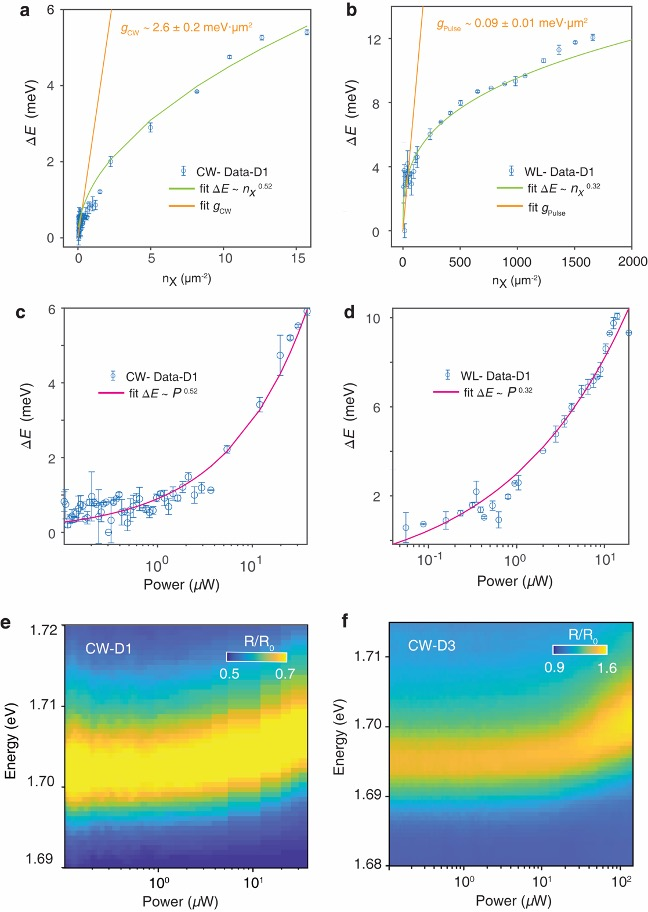
\includegraphics[width=0.75\textwidth]{Figures/C5/Fig5_8.jpg} % 
\end{center}
\caption[Analysis of power-dependent blueshift of X$_A^+$ under CW laser (a, c) and white laser excitation (b, d).] 
{\textbf{Analysis of power-dependent blueshift of X$_A^+$ under CW laser (a, c) and white laser excitation (b, d).}
\textbf{a,b,} Extraction of interaction strength $g$ from \textbf{(a)} CW laser and \textbf{(b)} pulsed laser pumping induced X$_A^+$ blueshift vs. exciton density for D1. 
The exciton density is calculated from pump flux based on $n_X=P \alpha \tau/\hbar \omega$, where $P$ is the pump power, $\alpha$ is the absorption coefficient, $\tau$ is the lifetime of the Fermi polaron, $\hbar \omega$ is the photon energy. 
The Fermi polaron lifetime is assumed as 2 ps. 
The interaction strength is extracted from the linear fit of the $\Delta E$--$n_X$ curve in the low exciton density regime. 
The larger $g$ values under CW excitation could be related to the complex relaxation dynamics of the exciton populations and an overestimation of exciton density under pulsed excitation. 
We also fit the blue shift amount as $\Delta E = a \cdot n_X^{(b)}$ over the entire data range. 
The fitting for CW laser and pulsed laser shows a sublinear response for X$_A^+$ as polaron density. 
The hole doping density is kept at $8 \times 10^{12}$ cm$^{-2}$. 
\textbf{c, d,} The same data as shown in \textbf{a, b,} plotted on semilog scale, with power as the x-axis. 
\textbf{e, f,} Power-dependent blueshift of X$_A^+$ under CW laser for \textbf{e,} device D1 and \textbf{f,} device D3. 
All error bars in \textbf{a-d} represent the variance of fitting peak energy.
}
\label{fig.5.8}
\end{figure}
\end{quote}
\renewcommand{\baselinestretch}{2}
\small\normalsize
% %///////////////////////
%////////////////////////////Figure Panel//////////////////
%Fig.5.9--------------
\renewcommand{\baselinestretch}{1}
\small\normalsize
\begin{quote}
\begin{figure}
\begin{center}
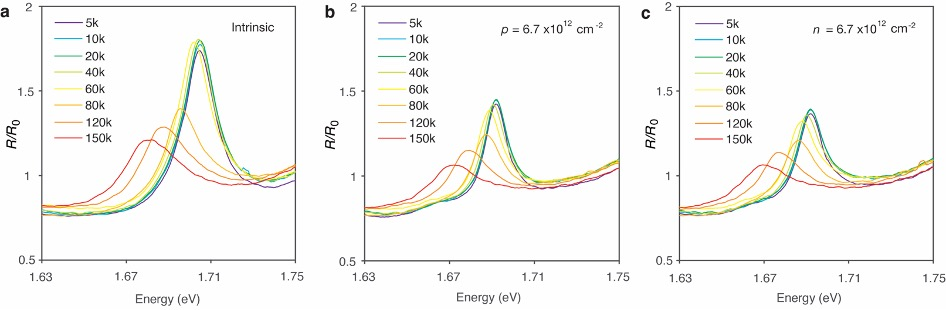
\includegraphics[width=1\textwidth]{Figures/C5/Fig5_9.jpg} % 
\end{center}
\caption[Temperature-dependent reflectance spectra of the trilayer under a constant doping density under zero electric field.] 
{\textbf{Temperature-dependent reflectance spectra of the trilayer under a constant doping density under zero electric field.}
In all cases, which include \textbf{(a)} intrinsic, \textbf{(b)} hole-doping, and \textbf{(c)} electron-doping, we observe strong redshift with increasing temperatures. Therefore, the observed nonlinearity, which corresponds to exciton blueshift, cannot be described as simple laser heating effects.}
\label{fig.5.9}
\end{figure}
\end{quote}
\renewcommand{\baselinestretch}{2}
\small\normalsize
% %///////////////////////

\section{Discussions}
The observed optical nonlinearity and their doping dependence cannot be simply explained by heating or carrier injection from the laser since both effects result in redshift of the intralayer excitons (Figures~\ref{fig.5.5}a and~\ref{fig.5.9}). 
Therefore, we examine how the interactions among the elementary excitations in the systems, \textit{i.e.}, intralayer excitons X$_A$, momentum-indirect excitons X$_I$, and free carriers, may give rise to the observed nonlinearity.

\subsection{Estimation of exciton interaction strength}
First, we extract a large interaction strength $g \sim 2~\mathrm{meV}\,\mu\mathrm{m}^{2}$ from the linear fit of energy blueshift vs.\ X$_A^+$ density at low power~\cite{ref30} (Figure~\ref{fig.5.8}). 
It is apparent that excitonic interactions (i.e.\ between X$_A$--X$_A$ and X$_A$--X$_I$) alone cannot produce the observed nonlinearity. 
On the one hand, the X$_A$--X$_A$ interactions among intralayer excitons are repulsive but weak, which scales linearly with density with a coefficient of $g_{\mathrm{ex}}\sim \alpha E_B R^{2}\sim 1.9~\mu\mathrm{eV}\,\mu\mathrm{m}^{2}$, where $\alpha$ is a constant ($\sim 6$), $E_B \approx 100~\mathrm{meV}$ is the exciton binding energy and $R$ ($\sim 1.78~\mathrm{nm}$) denotes the exciton Bohr radius in trilayers~\cite{ref31}. 
Given the short lifetime of X$_A$ ($\sim$picoseconds)~\cite{ref32,ref33} and thus the small density ($\sim 10^{9}~\mathrm{cm}^{-2}$), the amount of blueshift is expected to be orders of magnitude smaller than the experimental values (and comparable to monolayers and bilayers~\cite{ref20,ref31}). 
On the other hand, although X$_A$ can acquire a dipole moment via its hybridization with IX$_D$ and experience X$_A$--X$_I$ dipolar interaction with X$_I$, such interactions should have persisted in the intrinsic and electron-doped regime. 
Furthermore, we estimate an upper limit of dipolar interaction strength. 
We note that to the first order, there should be zero net dipoles and weak dipolar interactions under symmetric gating. 
However, the emergence of local net dipoles is plausible due to spontaneous symmetry breaking. 
Considering this, we calculate an upper limit for the dipolar interactions, assuming all dipoles are aligned. 
Using a parallel plate model, the dipolar interaction strength is given by $g_d=\frac{e^{2} d}{\varepsilon_{0}\,\varepsilon_{\mathrm{TMD}}}$, where $e d$ is the dipole moment of X$_A$. 
This dipole moment, $e d$, acquired from the hybridization with IX$_D$, can be estimated from the composition percentage of each exciton species in the coupled oscillator model. 
The value peaks when X$_A$ become degenerate with IX$_D$ reaching $\sim 0.7~\mathrm{nm}\cdot e$, and leading to an estimated dipolar interaction strength of $g_d \sim 1.8~\mu\mathrm{eV}\,\mu\mathrm{m}^{2}$, orders of magnitude smaller than the experimental interaction strength $g$. 
This conclusion is supported by the experimental observation of much weaker nonlinearity of X$_I$ than X$_A^+$, even when X$_I$ is fully polarized by an external electric field (see Figure~\ref{fig.5.10}).

%////////////////////////////Figure Panel//////////////////
%Fig.5.10--------------
\renewcommand{\baselinestretch}{1}
\small\normalsize
\begin{quote}
\begin{figure}
\begin{center}
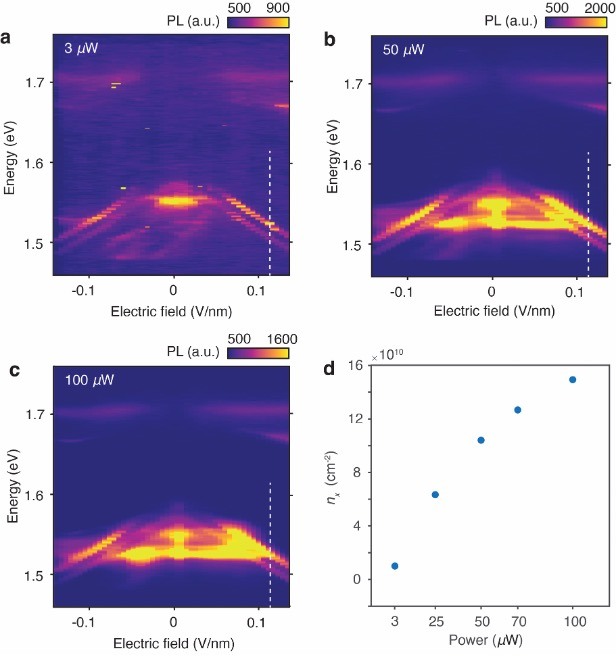
\includegraphics[width=0.75\textwidth]{Figures/C5/Fig5_10.jpg} % 
\end{center}
\caption[Estimation of X$_I$ density as a function of pump power.] 
{\textbf{Estimation of X$_I$ density as a function of pump power.}
\textbf{a-c,} Electric field-dependent PL map under different pump power \textbf{(a)} 3 $\mu$W, \textbf{(b)} 50 $\mu$W, \textbf{(c)} 100 $\mu$W at the trilayer region. 
At an electric field of 0.12 V/nm, a maximum blue shift in a value of 3.3 meV of the X$_I$ is observed. 
\textbf{(f)} X$_I$ exciton density inferred from the above X$_I$ blueshift under an applied electric field of 0.12 V/nm.
}
\label{fig.5.10}
\end{figure}
\end{quote}
\renewcommand{\baselinestretch}{2}
\small\normalsize
% %///////////////////////

\subsection{Nonlinearity due to valley polarization}
Therefore, we attribute the observed nonlinearity to a valley polarization created from the interactions between X$_A$ and free carriers. 
In particular, excitons created by optical pumping may induce a nonequilibrium valley population imbalance of resident carriers between $K$ and $\Gamma$ valleys, via mechanisms such as exciton--carrier scattering~\cite{ref34,ref35}. 
Importantly, under zero electric field, the energy difference between $K$ and $\Gamma$ valleys is rather small in trilayers~\cite{ref22}, on the order of tens of millielectronvolts, based on first-principle calculations and transport studies (Figure~\ref{fig.5.11}a). 
As a result, electrostatically doped holes at the $\Gamma$ point could be efficiently scattered into the $K$ valley by excitons such as X$_A$ and X$_I$, via Coulombic and exchange interactions~\cite{ref34,ref35} (Figure~\ref{fig.5.11}b). 
This net accumulation of valley population at $K$ (and $K'$) induces phase-space filling and, consequently, the observed blueshift of X$_A^+$. 
Such a scattering process would also introduce additional dephasing, which explains the increase in the X$_A^+$ linewidth.

%////////////////////////////Figure Panel//////////////////
%Fig.5.11--------------
\renewcommand{\baselinestretch}{1}
\small\normalsize
\begin{quote}
\begin{figure}
\begin{center}
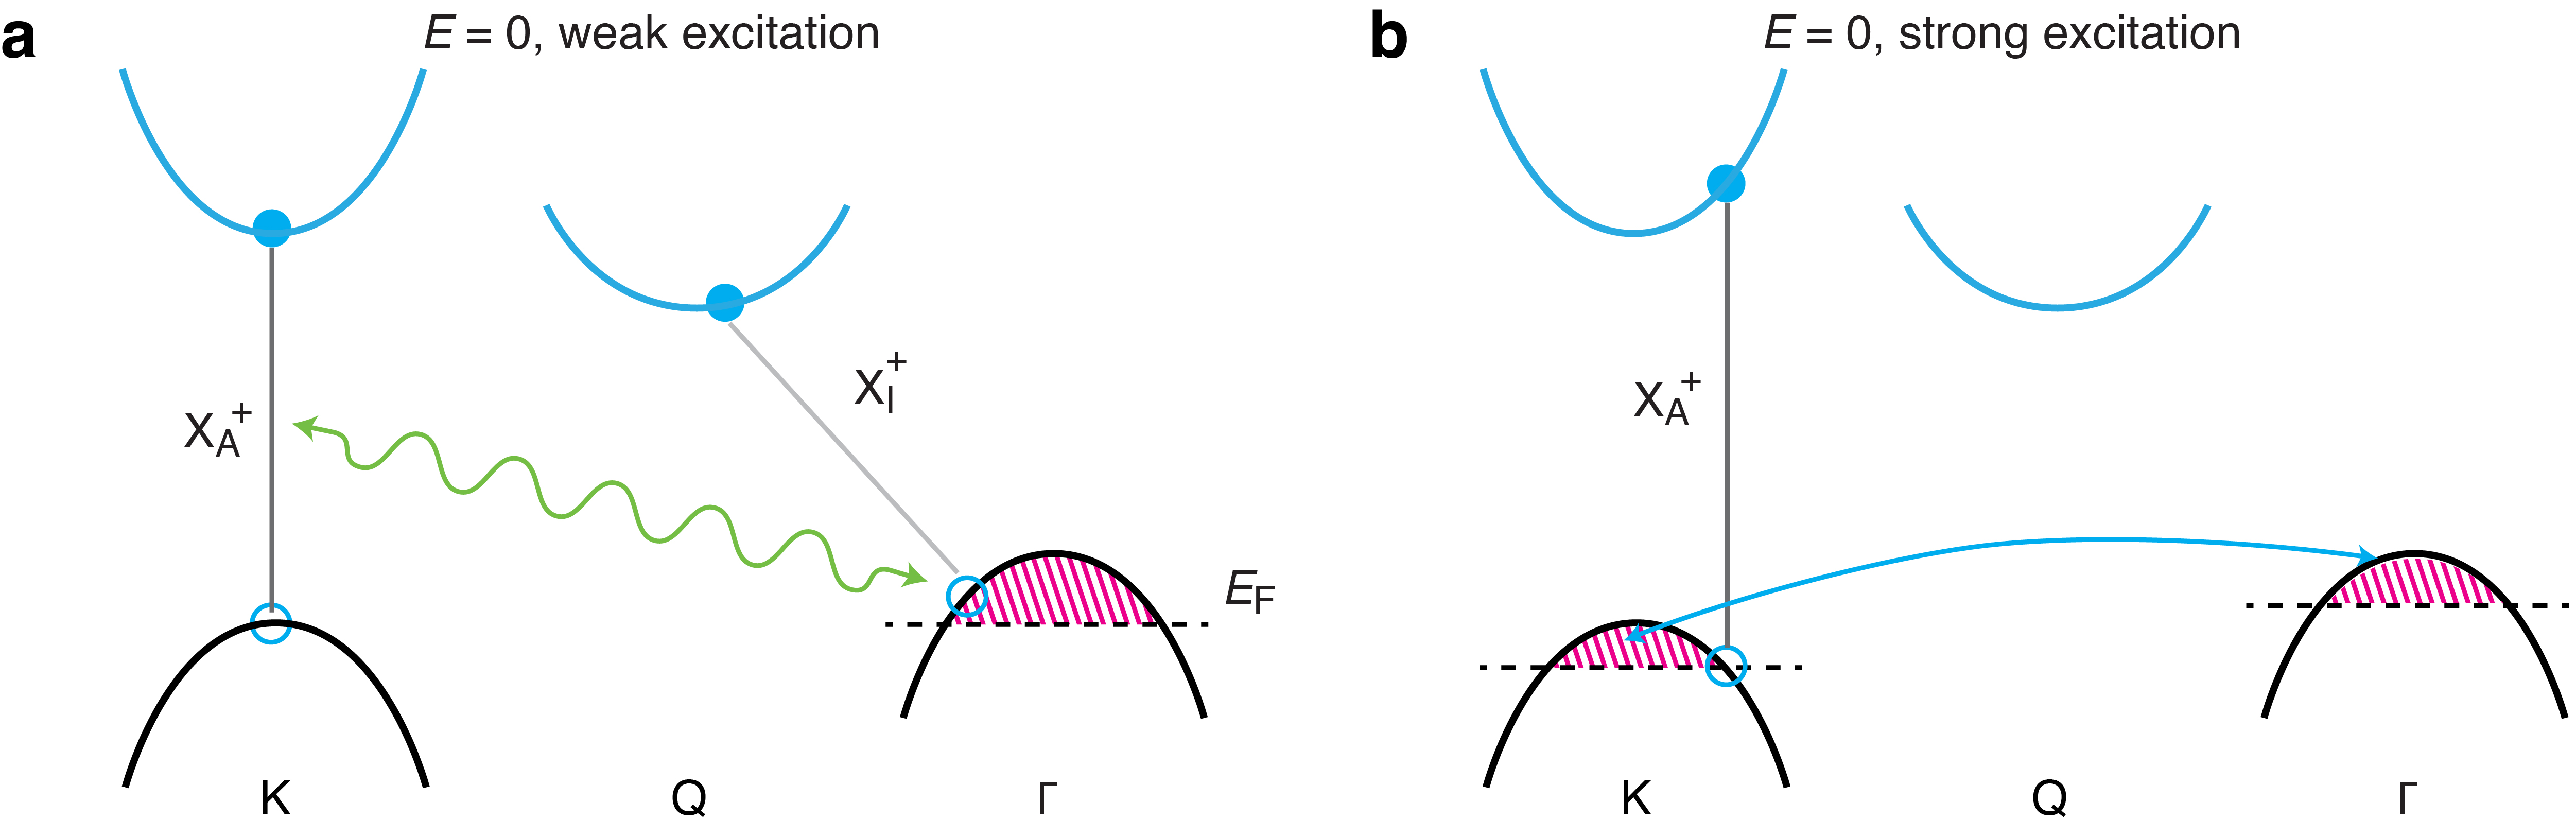
\includegraphics[width=1\textwidth]{Figures/C5/Fig5_11.jpg} % 
\end{center}
\caption[Optically induced valley polarization.] 
{\textbf{Optically induced valley polarization.}
\textbf{a, }Optical excitation generates both momentum direct intralayer X$_A^+$  and momentum indirect XI of higher population. 
Intralayer Fermi polaron X$_A^+$ can interact with X$_I$ and the free holes in the system. 
\textbf{b,} Under strong optical excitation, the interaction between intralayer excitons and free charges can induce a population transfer of carriers from the $\Gamma$ to the $K$ valley. 
The energy difference between $\Gamma$ and $K$ is small. 
The additional free carriers in K valley leads to phase space filling and optically induced blueshift of X$_A^+$. We note that in this nonequilibrium state, the dashed lines do not represent the Fermi level but are indications for the carrier population.
}
\label{fig.5.11}
\end{figure}
\end{quote}
\renewcommand{\baselinestretch}{2}
\small\normalsize
% %///////////////////////
Meanwhile, the oscillator strength remains unchanged at low excitation power, since it depends on the total doping level, but decreases at higher power due to saturation. 
In addition to the exciton--carrier scattering, the net valley polarization may also be created by the electric field induced by optical pumping. 
For instance, it has been suggested in bilayer TMDs that the generation of dipolar X$_I$ excitons may create a non-zero displacement field due to spontaneous symmetry breaking~\cite{ref1}. 
Such a displacement field can introduce a relative energy shift between $K$ and $\Gamma$ valleys~\cite{ref22}, thus creating a valley polarization. 
To further investigate such possible valley polarization, we probe the population of the resident carriers in the $K$ and $K'$ valleys under circularly polarized resonant excitation. 
As shown in Figure~\ref{fig.5.12}, we observe a stronger blueshift of X$_A^+$ in the $K$ than in the $K'$ valley when exciting excitons in the $K$ valley, consistent with our optically induced valley polarization picture.

%////////////////////////////Figure Panel//////////////////
%Fig.5.12--------------
\renewcommand{\baselinestretch}{1}
\small\normalsize
\begin{quote}
\begin{figure}
\begin{center}
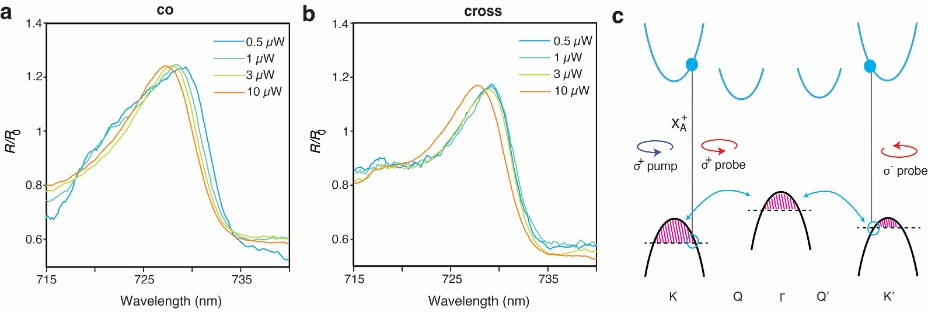
\includegraphics[width=1\textwidth]{Figures/C5/Fig5_12.jpg} % 
\end{center}
\caption[Valley-polarized holes under resonant circularly polarized excitation.] 
{\textbf{Valley-polarized holes under resonant circularly polarized excitation.} \textbf{a, b,} Power-dependent blueshift of X$_A^+$ under resonant pumping with \textbf{(a)} $\sigma^+/\sigma^+$ (pumping and probing $K$ valley) and \textbf{(b)} $\sigma^+/\sigma^-$ configuration (pumping $K$, while probing $K'$ valley) when the sample is hole-doped. 
We observe a stronger blueshift of X$_A^+$ in \textbf{(a)}. 
In particular, we observe a $\sim$1.3~nm blueshift under 3~$\mu$W pump when the pump and probe are co-polarized and no obvious shift in the cross-polarized case. 
Further increasing the pumping power to 10~$\mu$W leads to a blueshift in the cross-polarized setup, albeit still being smaller than the co-polarized case, which suggests the holes are partially polarized in $K$ vs.\ $K'$. 
The data is acquired from device D3. 
\textbf{c,} Nonequilibrium hole accumulation in $K$ and $K'$ valleys induced by selective valley pumping with a circularly polarized excitation. 
The resulting population imbalance between $K$ and $K'$ causes different amounts of blueshift in X$_A^+$ nonlinearity between the two valleys.   
}
\label{fig.5.12}
\end{figure}
\end{quote}
\renewcommand{\baselinestretch}{2}
\small\normalsize
% %///////////////////////
The proposed valley polarization mechanism also explains the strong electron--hole asymmetry of optical nonlinearity. 
Intrinsic trilayer WSe$_2$ exhibit weak nonlinearity, since no valley polarization can be created without resident carriers. 
In the electron-doped case, the valley polarization of resident carriers is prevented by the much larger energy splitting, on the order of hundreds of millielectronvolts, between $Q$ (band minimum) and the $K$ valleys (where X$_A$ resides) in the conduction band~\cite{ref22}. 
We also briefly note that in TMD monolayers, optical pumping with circularly polarized light can polarize carriers in $K$ vs.\ $K'$ valleys~\cite{ref32,ref33,ref34,ref35,ref36,ref37,ref38}. 
The generation of valley imbalance in monolayers has been attributed to mechanisms such as different inter-valley vs.\ intra-valley carrier relaxation rates, and different indirect excitons and spin-forbidden dark excitons relaxation rates~\cite{ref39,ref40}. 
Unlike in monolayers, where a spin flip of carriers is required for scattering between $K$ and $K'$ valleys, the $\Gamma$ point is spin-degenerate so that the intervalley scattering between $K$ and $\Gamma$ in trilayers can happen via a spin-conserving process, such as direct Coulomb and exchange interactions between holes and excitons. 
We note that X$_I$ likely plays a crucial role in exciton--electron scattering owing to their larger population than X$_A$ (see Figure~\ref{fig.5.10} for estimated X$_I$ density). 
Since relaxation processes of X$_A \rightarrow$ X$_I$ and X$_I \rightarrow$ ground state both involve finite momentum transfer, they can facilitate the valley polarization process via exciton--carrier scattering. 
This suggests that the dynamics of valley polarization could occur at a timescale similar to the X$_I$ lifetime, on the order of nanoseconds, which may explain our observation of weaker nonlinearity created by the pulsed laser compared to CW excitation with the same peak power (Figure~\ref{fig.5.8}).

To further corroborate our hypothesis, we control the relative energies of $\Gamma$ and $K$ valleys by applying an external electric field~\cite{ref20,ref22}, and study the resulting changes in both the energies and optical nonlinearity of Fermi polarons. 

First, we measure the reflectance of the X$_A^+$ and X$_A^-$ as we change the electric field under fixed doping levels (Figures~\ref{fig.5.13}a,b). 
With an increasing field, the energy of the X$_A^+$ blueshifts at a smaller electric field and then switches to a redshift above an electric field of $\sim$0.05~V/nm (Figure~\ref{fig.5.13}a). 
The electric field shifts the valence band maximum from $\Gamma$ to $K$ due to the distinct orbital characters of the eigenstates~\cite{ref22}. 
While the eigenstate at $K$ becomes layer-polarized with higher energies with the field, the wavefunction at the $\Gamma$ point features large interlayer coupling with only small energy changes under the field~\cite{ref22}.
This shift from $\Gamma$ to $K$ leads to more phase-space filling in $K$ and a blueshift of X$_A^+$, consistent with our proposed mechanism for optical nonlinearity (Figure~\ref{fig.5.14}). 
Above an electric field of $\sim$0.05~V/nm, X$_A^+$ begins to redshift. 
This electric field is comparable to the critical field under which the band edge shifts from $\Gamma$ to $K$, as determined from transport studies~\cite{ref22} (note that the literature-reported field differs from our definition by a factor of the relative dielectric constant). 

In stark contrast, the energy shift of the X$_A^-$ is much smaller in the electron-doped region (Figure~\ref{fig.5.13}b), where the band edge remains at the $Q$ point. 
The small energy variation of X$_A^-$ can be explained by the avoided crossing, similar to the undoped case.

%////////////////////////////Figure Panel//////////////////
%Fig.5.13--------------
\renewcommand{\baselinestretch}{1}
\small\normalsize
\begin{quote}
\begin{figure}[htbp]
\begin{center}
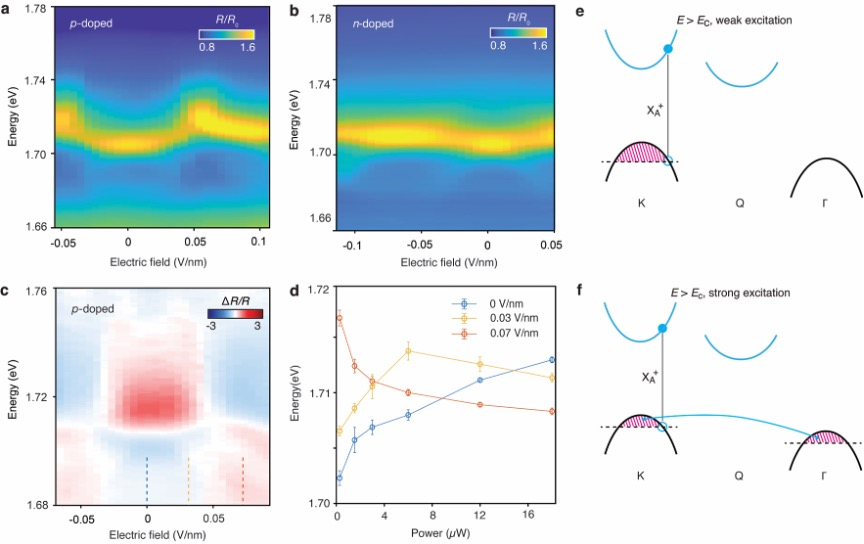
\includegraphics[width=1\textwidth]{Figures/C5/Fig5_13.jpg} % 
\end{center}
\caption[Electric-field dependent exciton energy and nonlinearity in homotrilayer WSe$_2$ at $T = 4$~K.] 
{\textbf{Electric-field dependent exciton energy and nonlinearity in homotrilayer WSe$_2$ at $T = 4$~K.} \textbf{a, b}, Electric-field dependence of the intralayer Fermi polaron reflectance contrast $R/R_{0}$ in trilayer with \textbf{(a)} hole and \textbf{(b)} electron doping density of $4.9 \times 10^{12}$~cm$^{-2}$. 
\textbf{c}, Reflectance change induced by a pulsed laser excitation of 12~$\mu$W power. 
The color map is obtained the same way as Figure~\ref{fig.5.6} d. 
Under a small electric field, X$_A^+$ shows a blueshift but it begins to redshift under excitation at higher electric fields. 
\textbf{d}, Line plots of the X$_A^+$ power-dependent peak shift under different electric fields. 
The X$_A^+$ shows a blueshift of $\sim$10~meV under zero applied electric field and a redshift of similar magnitude under large electric fields. 
The corresponding electric fields for these linecuts are indicated by the dashed lines in \textbf{(c)}. 
The error bars represent the uncertainty in determining the peak energy when fitting the reflection data. 
\textbf{e, f}, An electric field induces a shift of the valence band edge from $\Gamma$ to $K$ valley. 
Under strong optical pumping, a net valley polarization is induced by exciton--carrier scattering with increased carriers at the $\Gamma$ point, which leads to the optically induced redshift of X$_A^+$ at higher electric fields. 
In the nonequilibrium states, the dashed lines are used as indications for the carrier populations, and do not represent the Fermi level.}
\label{fig.5.13}
\end{figure}
\end{quote}
\renewcommand{\baselinestretch}{2}
\small\normalsize
% %/////////////////////// 

Intriguingly, the electric field also dramatically changes the nonlinear responses of X$_A^+$. 
As shown in Figure~\ref{fig.5.13}c, the reflectance change induced by optical pumping, $\Delta R/R$, shows a clear flip in the color contrast at $\sim$0.05~V/nm, which coincides with the crossover field between the blueshift and redshift of X$_A^+$ in Figure~\ref{fig.5.13}a. 
The magnitude of the blueshift and redshift is similar under the same excitation conditions, around 10~meV (Figure~\ref{fig.5.13}d). 
Such electric-field control of optical nonlinearity provides additional supporting evidence for our proposed mechanism involving valley polarization (Figures~\ref{fig.5.13} e,f). 
Figure~\ref{fig.5.13} e shows the modified band structure above the critical field~\cite{ref22}. 
Under optical excitation, the same exciton--hole scattering process can induce a population transfer of holes from $K$ to $\Gamma$, and reduce the X$_A^+$ energies (Figure~\ref{fig.5.13} f). 
This also explains the similar critical electric fields where both nonlinearity and electric-field susceptibility turn from blue- to redshift.

%////////////////////////////Figure Panel//////////////////
%Fig.5.14--------------
\vspace{2em}
\renewcommand{\baselinestretch}{2}
\small\normalsize
\begin{quote}
\begin{figure}[htbp]
\begin{center}
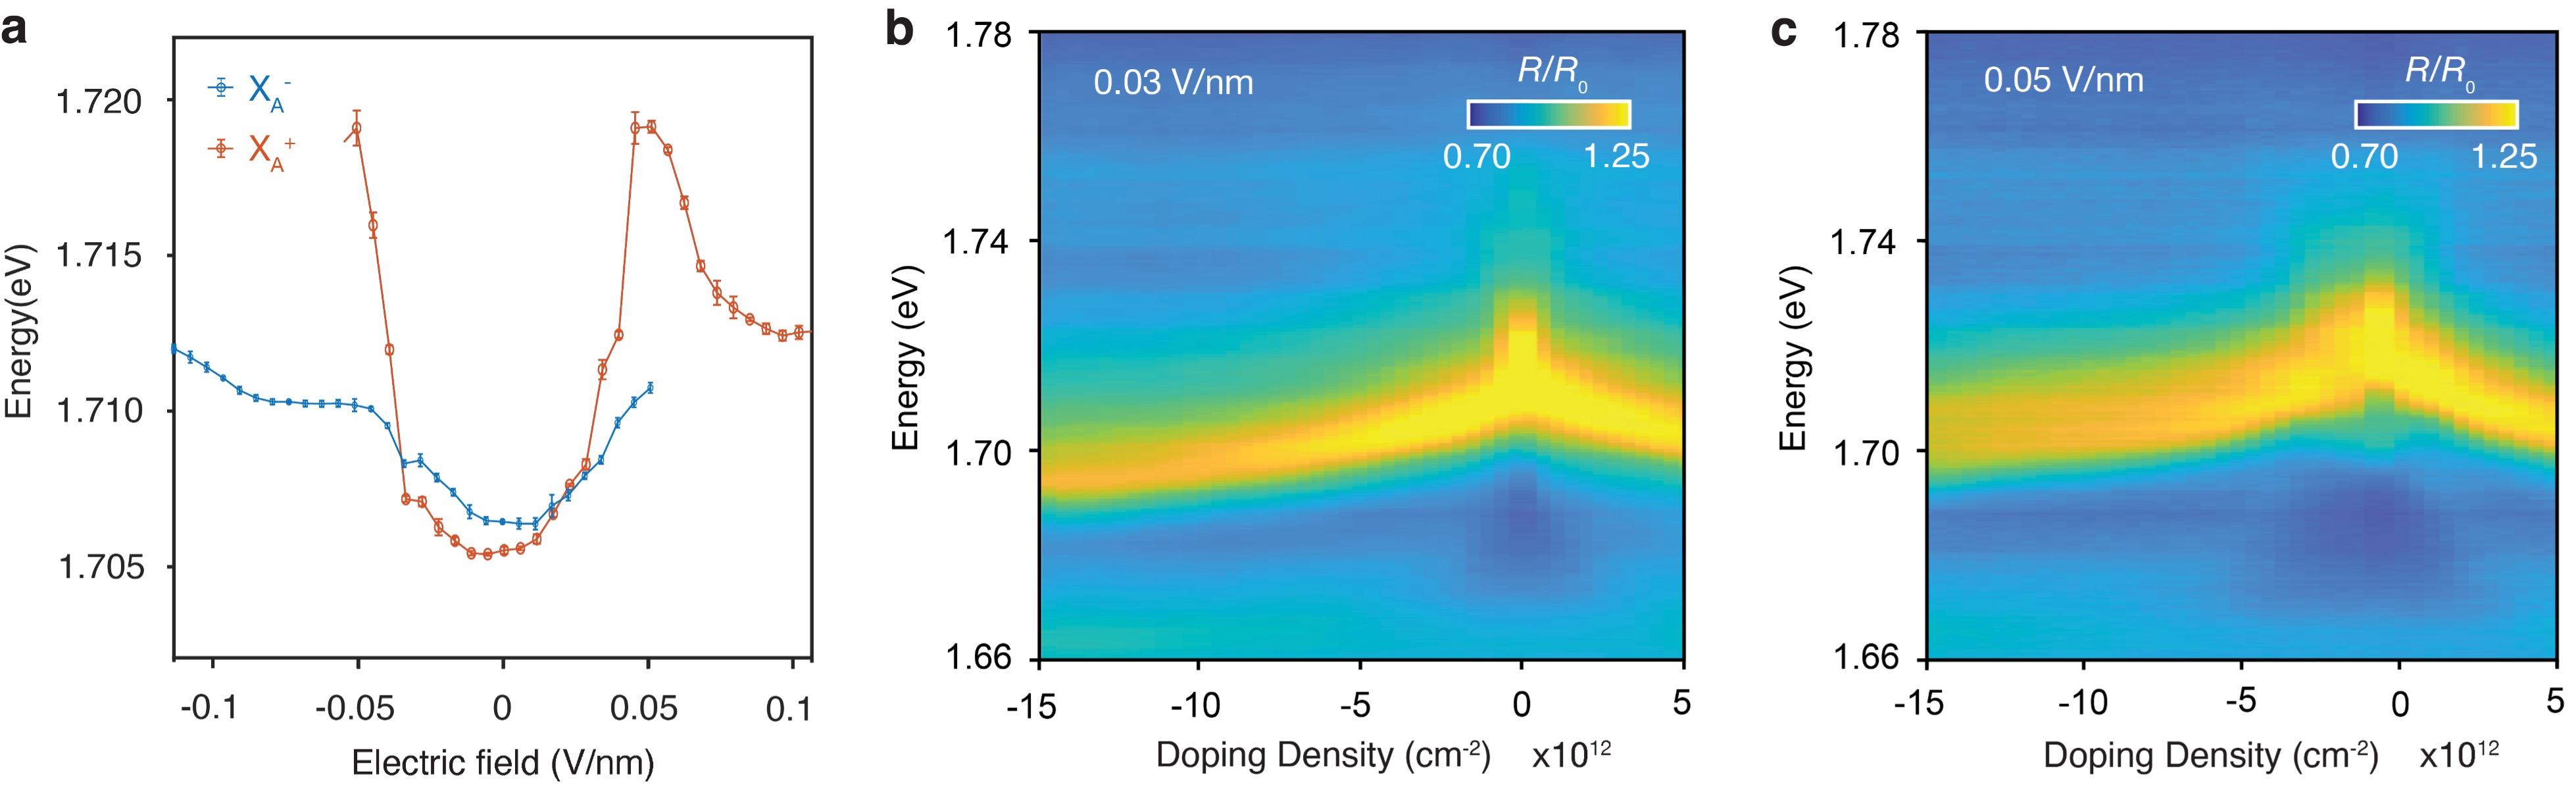
\includegraphics[width=1\textwidth]{Figures/C5/Fig5_14.jpg} % 
\end{center}
\caption[Electric-field tuning of Fermi polarons.] 
{\textbf{Electric-field tuning of Fermi polarons.} 
\textbf{a}, Energy shift of X$_A^-$ and X$_A^+$ with applied electric field at constant doping. 
The electron and hole doping densities are both kept at $4.9 \times 10^{12}$~cm$^{-2}$. 
The peak position is obtained by fitting the reflectance spectra with a Lorentzian model. 
The error bars represent the variance of the fitted peak energy.  
\textbf{b, c}, Doping dependence of the intralayer Fermi polaron reflectance contrast $R/R_{0}$ in trilayer with applied \textbf{(b)} 0.03~V/nm, \textbf{(c)} 0.05~V/nm electric field. 
The negative doping density represents the hole-doped side. 
An obvious blueshift and broadening of X$_A^+$ is observed on the hole side with increasing electric field, corresponding to additional phase-space filling due to the population transfer from $\Gamma$ to $K$ valleys. 
Such a shift is much weaker on the electron side.}
\label{fig.5.14}
\end{figure}
\end{quote}
\renewcommand{\baselinestretch}{2}
\small\normalsize
% %/////////////////////// 

\newpage
\section{Conclusions}
Our results demonstrating highly nonlinear excitons with large oscillator strengths open avenues for engineering exciton--carrier interactions in atomically thin heterostructures to explore strongly interacting many-body physics and develop novel optoelectronics. 
By designing the atomic and electronic structures of the heterostructures, one may engineer the strong interactions between bright, dark excitons, and free charges~\cite{ref26}. 
The excitonic and free charge populations are highly tunable, and elucidating the complex interactions between intralayer, interlayer excitons, and charges will be of significant future interest for studying many-body physics in a hybrid Fermi--Bose system~\cite{ref41,ref42,ref43}, from both theoretical and experimental perspectives. 
These strongly interacting optical excitations can be used to realize active nonlinear metasurfaces based on spatial confinement of excitons by moiré superlattices and local electrostatic gates~\cite{ref44,ref45,ref46}. 
Combining strong nonlinearity with spatial confinement could also further boost nonlinearity and allow exploring quantum optical effects, including nonclassical light sources and few-photon nonlinearity~\cite{ref11,ref47}. 
While current experiments require $10^3$--$10^4$ photons to shift the resonance by a linewidth, improving materials quality and engineering the photonic environment could lower the required photon count significantly by reducing the Fermi polaron linewidth. 
Finally, the demonstrated optical control of exciton resonances could enable novel nonlinear optoelectronic devices such as all-optical switching, nonlinear optomechanical resonators~\cite{ref48,ref49}, and optical limiting devices~\cite{ref4,ref50}.